% ------------------------------------------------------------
% LaTeX Template für die DHBW zum Schnellstart!
% Original: https://github.wdf.sap.corp/vtgermany/LaTeX-Template-DHBW
% ------------------------------------------------------------
% ---- Präambel mit Angaben zum Dokument
\documentclass[
	fontsize=12pt,           % Leitlinien sprechen von Schriftgröße 12.
	paper=A4,
	twoside=false,
	listof=totoc,            % Tabellen- und Abbildungsverzeichnis ins Inhaltsverzeichnis
	bibliography=totoc,      % Literaturverzeichnis ins Inhaltsverzeichnis aufnehmen
	titlepage,               % Titlepage-Umgebung anstatt \maketitle
	headsepline,             % horizontale Linie unter Kolumnentitel
	abstract,              % Überschrift einschalten, Abstract muss in {abstract}-Umgebung stehen
]{scrreprt}                  % Verwendung von KOMA-Report
\usepackage[utf8]{inputenc}  % UTF8 Encoding einschalten
\usepackage[ngerman]{babel}  % Neue deutsche Rechtschreibung
\usepackage[T1]{fontenc}     % Ausgabe von westeuropäischen Zeichen (auch Umlaute)
\usepackage{microtype}       % Trennung von Wörtern wird besser umgesetzt
\usepackage{lmodern}         % Nicht-gerasterte Schriftarten (bei MikTeX erforderlich)
\usepackage{graphicx}        % Einbinden von Grafiken erlauben
\usepackage{wrapfig}         % Grafiken fließend im Text
\usepackage{setspace}        % Zeilenabstand \singlespacing, \onehalfspaceing, \doublespacing
\usepackage[
	%showframe,                % Ränder anzeigen lassen
	left=2.7cm, right=2.5cm,
	top=2.5cm,  bottom=2.5cm,
	includeheadfoot
]{geometry}                      % Seitenlayout einstellen
\usepackage{scrlayer-scrpage}    % Gestaltung von Fuß- und Kopfzeilen
\usepackage{acronym}             % Abkürzungen, Abkürzungsverzeichnis
\usepackage{titletoc}            % Anpassungen am Inhaltsverzeichnis
\contentsmargin{0.75cm}          % Abstand im Inhaltsverzeichnis zw. Punkt und Seitenzahl
\usepackage[                     % Klickbare Links (enth. auch "nameref", "url" Package)
  hidelinks,                     % Blende die "URL Boxen" aus.
  breaklinks=true                % Breche zu lange URLs am Zeilenende um
]{hyperref}
\usepackage[hypcap=true]{caption}% Anker Anpassung für Referenzen
\urlstyle{same}                  % Aktuelle Schrift auch für URLs
% Anpassung von autoref für Gleichungen (ergänzt runde Klammern) und Algorithm.
% Anstatt "Listing" kann auch z.B. "Code-Ausschnitt" verwendet werden. Dies sollte
% jedoch synchron gehalten werden mit \lstlistingname (siehe weiter unten).
\addto\extrasngerman{%
	\def\equationautorefname~#1\null{Gleichung~(#1)\null}
	\def\lstnumberautorefname{Zeile}
	\def\lstlistingautorefname{Listing}
	\def\algorithmautorefname{Algorithmus}
	% Damit einheitlich "Abschnitt 1.2[.3]" verwendet wird und nicht "Unterabschnitt 1.2.3"
	% \def\subsectionautorefname{Abschnitt}
}

% ---- Abstand verkleinern von der Überschrift 
\renewcommand*{\chapterheadstartvskip}{\vspace*{.5\baselineskip}}

% Hierdurch werden Schusterjungen und Hurenkinder vermieden, d.h. einzelne Wörter
% auf der nächsten Seite oder in einer einzigen Zeile.
% LaTeX kann diese dennoch erzeugen, falls das Layout ansonsten nicht umsetzbar ist.
% Diese Werte sind aber gute Startwerte.
\widowpenalty10000
\clubpenalty10000

% ---- Für das Quellenverzeichnis
\usepackage[
	backend = biber,                % Verweis auf biber
	language = auto,
	style = numeric,                % Nummerierung der Quellen mit Zahlen
	sorting = none,                 % none = Sortierung nach der Erscheinung im Dokument
	sortcites = true,               % Sortiert die Quellen innerhalb eines cite-Befehls
	block = space,                  % Extra Leerzeichen zwischen Blocks
	hyperref = true,                % Links sind klickbar auch in der Quelle
	%backref = true,                % Referenz, auf den Text an die zitierte Stelle
	bibencoding = auto,
	giveninits = true,              % Vornamen werden abgekürzt
	doi=false,                      % DOI nicht anzeigen
	isbn=false,                     % ISBN nicht anzeigen
    alldates=short                  % Datum immer als DD.MM.YYYY anzeigen
]{biblatex}
\addbibresource{Inhalt/literatur.bib}
\setcounter{biburlnumpenalty}{3000}     % Umbruchgrenze für Zahlen
\setcounter{biburlucpenalty}{6000}      % Umbruchgrenze für Großbuchstaben
\setcounter{biburllcpenalty}{9000}      % Umbruchgrenze für Kleinbuchstaben
\DeclareNameAlias{default}{family-given}  % Nachname vor dem Vornamen
\AtBeginBibliography{\renewcommand{\multinamedelim}{\addslash\space
}\renewcommand{\finalnamedelim}{\multinamedelim}}  % Schrägstrich zwischen den Autorennamen
\DefineBibliographyStrings{german}{
  urlseen = {Einsichtnahme:},                      % Ändern des Titels von "besucht am"
}
\usepackage[babel,german=quotes]{csquotes}         % Deutsche Anführungszeichen + Zitate


% ---- Für Mathevorlage
\usepackage{amsmath}    % Erweiterung vom Mathe-Satz
\usepackage{amssymb}    % Lädt amsfonts und weitere Symbole
\usepackage{MnSymbol}   % Für Symbole, die in amssymb nicht enthalten sind.


% ---- Für Quellcodevorlage
\usepackage{scrhack}                    % Hack zur Verw. von listings in KOMA-Script
\usepackage{listings}                   % Darstellung von Quellcode
\usepackage{xcolor}                     % Einfache Verwendung von Farben
% -- Eigene Farben für den Quellcode
\definecolor{JavaLila}{rgb}{0.4,0.1,0.4}
\definecolor{JavaGruen}{rgb}{0.3,0.5,0.4}
\definecolor{JavaBlau}{rgb}{0.0,0.0,1.0}
\definecolor{ABAPKeywordsBlue}{HTML}{6000ff}
\definecolor{ABAPCommentGrey}{HTML}{808080}
\definecolor{ABAPStringGreen}{HTML}{4da619}
\definecolor{PyKeywordsBlue}{HTML}{0000AC}
\definecolor{PyCommentGrey}{HTML}{808080}
\definecolor{PyStringGreen}{HTML}{008080}
% -- Farben für ABAP CDS
\definecolor{CDSString}{HTML}{FF8C00}
\definecolor{CDSKeywords}{HTML}{6000ff}
\definecolor{CDSAnnotation}{HTML}{00BFFF}
\definecolor{CDSComment}{HTML}{808080}
\definecolor{CDSFunc}{HTML}{FF0000}

% -- Default Listing-Styles

\lstset{
	% Das Paket "listings" kann kein UTF-8. Deswegen werden hier 
	% die häufigsten Zeichen definiert (ä,ö,ü,...)
	literate=%
		{á}{{\'a}}1 {é}{{\'e}}1 {í}{{\'i}}1 {ó}{{\'o}}1 {ú}{{\'u}}1
		{Á}{{\'A}}1 {É}{{\'E}}1 {Í}{{\'I}}1 {Ó}{{\'O}}1 {Ú}{{\'U}}1
		{à}{{\`a}}1 {è}{{\`e}}1 {ì}{{\`i}}1 {ò}{{\`o}}1 {ù}{{\`u}}1
		{À}{{\`A}}1 {È}{{\'E}}1 {Ì}{{\`I}}1 {Ò}{{\`O}}1 {Ù}{{\`U}}1
		{ä}{{\"a}}1 {ë}{{\"e}}1 {ï}{{\"i}}1 {ö}{{\"o}}1 {ü}{{\"u}}1
		{Ä}{{\"A}}1 {Ë}{{\"E}}1 {Ï}{{\"I}}1 {Ö}{{\"O}}1 {Ü}{{\"U}}1
		{â}{{\^a}}1 {ê}{{\^e}}1 {î}{{\^i}}1 {ô}{{\^o}}1 {û}{{\^u}}1
		{Â}{{\^A}}1 {Ê}{{\^E}}1 {Î}{{\^I}}1 {Ô}{{\^O}}1 {Û}{{\^U}}1
		{œ}{{\oe}}1 {Œ}{{\OE}}1 {æ}{{\ae}}1 {Æ}{{\AE}}1 {ß}{{\ss}}1
		{ű}{{\H{u}}}1 {Ű}{{\H{U}}}1 {ő}{{\H{o}}}1 {Ő}{{\H{O}}}1
		{ç}{{\c c}}1 {Ç}{{\c C}}1 {ø}{{\o}}1 {å}{{\r a}}1 {Å}{{\r A}}1
		{€}{{\euro}}1 {£}{{\pounds}}1 {«}{{\guillemotleft}}1
		{»}{{\guillemotright}}1 {ñ}{{\~n}}1 {Ñ}{{\~N}}1 {¿}{{?`}}1,
	breaklines=true,        % Breche lange Zeilen um 
	breakatwhitespace=true, % Wenn möglich, bei Leerzeichen umbrechen
	% Symbol für Zeilenumbruch einfügen
	prebreak=\raisebox{0ex}[0ex][0ex]{\ensuremath{\rhookswarrow}},
	postbreak=\raisebox{0ex}[0ex][0ex]{\ensuremath{\rcurvearrowse\space}},
	tabsize=4,                                 % Setze die Breite eines Tabs
	basicstyle=\ttfamily\small,                % Grundsätzlicher Schriftstyle
	columns=fixed,                             % Besseres Schriftbild
	numbers=left,                              % Nummerierung der Zeilen
	%frame=single,                             % Umrandung des Codes
	showstringspaces=false,                    % Keine Leerzeichen hervorheben
	keywordstyle=\color{blue},
	ndkeywordstyle=\bfseries\color{darkgray},
	identifierstyle=\color{black},
	commentstyle=\itshape\color{JavaGruen},   % Kommentare in eigener Farbe
	stringstyle=\color{JavaBlau},             % Strings in eigener Farbe,
	captionpos=b,                             % Bild*unter*schrift
	xleftmargin=5.0ex
}

% ---- Eigener JAVA-Style für den Quellcode
\renewcommand{\ttdefault}{pcr}               % Schriftart, welche auch fett beinhaltet
\lstdefinestyle{EigenerJavaStyle}{
	language=Java,                             % Syntax Highlighting für Java
	%frame=single,                             % Umrandung des Codes
	keywordstyle=\bfseries\color{JavaLila},    % Keywords in eigener Farbe und fett
	commentstyle=\itshape\color{JavaGruen},    % Kommentare in eigener Farbe und italic
	stringstyle=\color{JavaBlau}               % Strings in eigener Farbe
}

% ---- Eigener ABAP-Style für den Quellcode
\renewcommand{\ttdefault}{pcr}
\lstdefinestyle{EigenerABAPStyle}{
	language=[R/3 6.10]ABAP,
	morestring=[b]\|,                          % Für Pipe-Strings
	morestring=[b]\`,                          % für Backtick-Strings
	keywordstyle=\bfseries\color{ABAPKeywordsBlue},
	commentstyle=\itshape\color{ABAPCommentGrey},
	stringstyle=\color{ABAPStringGreen},
	tabsize=2,
	morekeywords={
		types,
		@data,
		as,
		lower,
		start,
		selection,
		order,
		by,
		inner,
		join,
		key,
		end,
		cast
	}
}

% ---- Eigener Python-Style für den Quellcode
\renewcommand{\ttdefault}{pcr}
\lstdefinestyle{EigenerPythonStyle}{
	language=Python,
	columns=flexible,
	keywordstyle=\bfseries\color{PyKeywordsBlue},
	commentstyle=\itshape\color{PyCommentGrey},
	stringstyle=\color{PyStringGreen}
}

%----- ABAP-CDS-View language
\lstdefinelanguage{ABAPCDS}{
	sensitive=false,
	%Keywords
	morekeywords={define,
		view,
		as,
		select,
		from,
		inner,
		join,
		on,
		key,
		case,
		when,
		then,
		else,
		end,
		true,
		false,
		cast,
		where,
		and,
		distinct,
		group,
		by,
		having,
		min,
		sum,
		max,
		count,
		avg
	},
	%Methoden
	morekeywords=[2]{
		div,
		currency\_conversion,
		dats\_days\_between,
		concat\_with\_space,
		dats\_add_days,
		dats\_is\_valid,
		dats\_add\_months,
		unit\_conversion,
		division,
		mod,
		abs,
		floor,
		ceil,
		round,
		concat,
		replace,
		substring,
		left,
		right,
		length
	},
	morecomment=[s][\color{CDSAnnotation}]{@}{:},
	morecomment=[l][\itshape\color{CDSComment}]{//},
	morecomment=[s][\itshape\color{CDSComment}]{/*}{*/},
	morestring=[b][\color{CDSString}]',
	keywordstyle=\bfseries\color{CDSKeywords},
	keywordstyle=[2]\color{CDSFunc}
}

  % Weitere Details sind ausgelagert

\usepackage{algorithm}                  % Für Algorithmen-Umgebung (ähnlich wie lstlistings Umgebung)
\usepackage{algpseudocode}              % Für Pseudocode. Füge "[noend]" hinzu, wenn du kein "endif",
                                        % etc. haben willst.

\makeatletter                           % Sorgt dafür, dass man @ in Namen verwenden kann.
                                        % Ansonsten gibt es in der nächsten Zeile einen Compilefehler.
\renewcommand{\ALG@name}{Algorithmus}   % Umbenennen von "Algorithm" im Header der Listings.
\makeatother                            % Zeichen wieder zurücksetzen
\renewcommand{\lstlistingname}{Listing} % Erlaubt das Umbenennen von "Listing" in anderen Titel.

% ---- Tabellen
\usepackage{booktabs}  % Für schönere Tabellen. Enthält neue Befehle wie \midrule
\usepackage{multirow}  % Mehrzeilige Tabellen
\usepackage{siunitx}   % Für SI Einheiten und das Ausrichten Nachkommastellen
\sisetup{locale=DE, range-phrase={~bis~}, output-decimal-marker={,}} % Damit ein Komma und kein Punkt verwendet wird.
\usepackage{xfrac} % Für siunitx Option "fraction-function=\sfrac"

% ---- Für Definitionsboxen in der Einleitung
\usepackage{amsthm}                     % Liefert die Grundlagen für Theoreme
\usepackage[framemethod=tikz]{mdframed} % Boxen für die Umrandung
% ---- Definition für Highlight Boxen

% ---- Grundsätzliche Definition zum Style
\newtheoremstyle{defi}
  {\topsep}         % Abstand oben
  {\topsep}         % Abstand unten
  {\normalfont}     % Schrift des Bodys
  {0pt}             % Einschub der ersten Zeile
  {\bfseries}       % Darstellung von der Schrift in der Überschrift
  {:}               % Trennzeichen zwischen Überschrift und Body
  {.5em}            % Abstand nach dem Trennzeichen zum Body Text
  {\thmname{#3}}    % Name in eckigen Klammern
\theoremstyle{defi}

% ------ Definition zum Strich vor eines Texts
\newmdtheoremenv[
  hidealllines = true,       % Rahmen komplett ausblenden
  leftline = true,           % Linie links einschalten
  innertopmargin = 0pt,      % Abstand oben
  innerbottommargin = 4pt,   % Abstand unten
  innerrightmargin = 0pt,    % Abstand rechts
  linewidth = 3pt,           % Linienbreite
  linecolor = gray!40,       % Linienfarbe
]{defStrich}{Definition}     % Name der des formats "defStrich"

% ------ Definition zum Eck-Kasten um einen Text
\newmdtheoremenv[
  hidealllines = true,
  innertopmargin = 6pt,
  linecolor = gray!40,
  singleextra={              % Eck-Markierungen für die Definition
    \draw[line width=3pt,gray!50,line cap=rect] (O|-P) -- +(1cm,0pt);
    \draw[line width=3pt,gray!50,line cap=rect] (O|-P) -- +(0pt,-1cm);
    \draw[line width=3pt,gray!50,line cap=rect] (O-|P) -- +(-1cm,0pt);
    \draw[line width=3pt,gray!50,line cap=rect] (O-|P) -- +(0pt,1cm);
  }
]{defEckKasten}{Definition}  % Name der des formats "defEckKasten"  % Weitere Details sind ausgelagert

% ---- Für Todo Notes
\usepackage{todonotes}
\setlength {\marginparwidth }{2cm}      % Abstand für Todo Notizen


% ---- Elektronische Version oder Gedruckte Version?
% ---- Unterschied: Die elektronische Version enthält keinen Platzhalter für die Unterschrift
\usepackage{ifthen}
\newboolean{e-Abgabe}
\setboolean{e-Abgabe}{true}    % false=gedruckte Fassung

% ---- Persönlichen Daten:
\newcommand{\titel}{Digital Nudging und Nutzerverhalten}
\newcommand{\titelheader}{Digital Nudging und Nutzerverhalten}
\newcommand{\arbeit}{Seminararbeit}
\newcommand{\studiengang}{Internationale Wirtschaftsinformatik (IBAIT)}
\newcommand{\studienjahr}{2020}
\newcommand{\autor}{Vorname Nachname}
\newcommand{\autorReverse}{Nachname, Vorname}
\newcommand{\verfassungsort}{Ludwigshafen}
\newcommand{\matrikelnr}{0000000}
\newcommand{\kurs}{IBAIT20}
\newcommand{\bearbeitungsmonat}{Januar 2018}
\newcommand{\abgabe}{02.12.2022}
\newcommand{\bearbeitungszeitraum}{01.10.2022 - 02.12.2022}
%\newcommand{\firmaName}{SAP SE}
%\newcommand{\firmaStrasse}{Dietmar-Hopp-Allee 16}
%\newcommand{\firmaPlz}{69190 Walldorf, Deutschland}
%\newcommand{\betreuerFirma}{B-Vorname B-Nachname}
%\newcommand{\betreuerDhbw}{DH-Vorname DH-Nachname}

% ---- Metainformation für das PDF Dokument
\hypersetup{
	pdftitle    = {\titel},
	pdfsubject  = {\arbeit},
	pdfauthor   = {\autor},
	%pdfkeywords = {Keywords angeben},
	pdfcreator  = {LaTeX},
	%pdfproducer = {in der Regel pdfTeX}
}

% ---- Definition der Kopf- und Fußzeilen
\clearpairofpagestyles                          % Löschen von LaTeX Standard
\automark[section]{chapter}                     % Füllen von section und chapter
\renewcommand*{\chaptermarkformat}{}            % Entfernt die Kapitelnummer
\renewcommand*{\sectionmarkformat}{}            % Entfernt die Sectionnummer
% Angaben [für "plain"]{für "scrheadings"}
\ihead[]{\titelheader}                          % Kopfzeile links
\chead[]{}                                      % Kopfzeile mitte
\ohead[]{\rightmark}                            % Kopfzeile rechts
\ifoot[]{}                                      % Fußzeile links
\cfoot*{\sffamily\pagemark}                     % Fußzeile mitte
\ofoot[]{}                                      % Fußzeile rechts
\KOMAoptions{
   headsepline = 0.2pt,                         % Liniendicke Kopfzeile
   footsepline = false                          % Liniendicke Fußzeile
}


% ---- Hilfreiches
\newcommand{\zB}{z.\,B. }   % "z.B." mit kleinem Leeraum dazwischen (ohne wäre nicht korrekt)
\newcommand{\dash}{d.\,h. }

\newcommand{\code}[1]{\texttt{#1}} % Ist einfacher zu schreiben als ständig \texttt und erlaubt
                                   % Änderungen im Nachhinein, wenn man z.B. Inline-Code anders stylen möchte.

% ---- Silbentrennung (falls LaTeX defaults falsch / nicht gewünscht sind)
\hyphenation{HANA}         % anstatt HA-NA
\hyphenation{Graph-Script} % anstatt GraphS-cript

% ---- Beginn des Dokuments
\begin{document}
\setlength{\parindent}{0pt}              % Keine Paragraphen Einrückung.
                                         % Dafür haben wir den Abstand zwischen den Paragraphen.
\setcounter{secnumdepth}{2}              % Nummerierungstiefe fürs Inhaltsverzeichnis
\setcounter{tocdepth}{1}                 % Tiefe des Inhaltsverzeichnisses. Ggf. so anpassen,
                                         % dass das Verzeichnis auf eine Seite passt.
\sffamily                                % Serifenlose Schrift verwenden.

% ---- Vorspann
% ------ Titelseite
\singlespacing
\thispagestyle{empty}
\begin{titlepage}
\enlargethispage{4cm}

\begin{figure}           % Logo vom Ausbildungsbetrieb und der DHBW
	% \vspace*{-5mm} % Sollte dein Titel zu lang werden, kannst du mit diesem "Hack" 
	%                  den Inhalt der Seite nach oben schieben.
	\begin{minipage}{0.49\textwidth}
		\flushleft
		
\includegraphics[height=1.8cm]{Bilder/Logos/Logo_SAP.pdf} 
	\end{minipage}
	\hfill
	\begin{minipage}{0.49\textwidth}
		\flushright
		
\includegraphics[height=1.8cm]{Bilder/Logos/Logo_HWG-Lu.jpg} 
	\end{minipage}
\end{figure} 
\vspace*{0.1cm}

\begin{center}
	\huge{\textbf{\titel}}\\[1.5cm]
	\Large{\textbf{\arbeit}}\\[0.5cm]
	\normalsize{as part of the examination for the degree\\[1ex] \textbf{Bachelor of Science (B.Sc.)}}\\[0.5cm]
	\Large{of \studiengang}\\[1ex]
	\normalsize{at the University of Business and Society}\\[1cm]
	\normalsize{by}\\[1ex] \Large{\textbf{\autor}} \\[1cm]
	% Hinweis: Manche Dozenten möchten einen Hinweis auf den Sperrvermerk auf der Titelseite.
	% \large{{\color{red}- Sperrvermerk -}}\\[1cm]
\end{center}

\begin{center}
	\vfill
	\begin{tabular}{ll}
		Abgabedatum:                     & \abgabe \\[0.2cm]
		Bearbeitungszeitraum:            & \bearbeitungszeitraum \\[0.2cm]
		Matrikelnummer, Kurs:            & \matrikelnr , \kurs \\[0.2cm]
		Ausbildungsfirma:                & \firmaName \\
		                                 & \firmaStrasse \\
		                                 & \firmaPlz \\[0.2cm]
		Betreuer der Ausbildungsfirma:   & \betreuerFirma \\[0.2cm]
		Gutachter der Dualen Hochschule: & \betreuerDhbw \\[2cm]
	\end{tabular} 
\end{center}
\end{titlepage}
  % Titelseite
\newcounter{savepage}
\pagenumbering{roman}                    % Römische Seitenzahlen
\onehalfspacing

% ------ Erklärung, Sperrvermerk, Abstact
\chapter*{Ehrenwörtliche Erklärung}
Wir erklären hiermit ehrenwörtlich, die vorliegende \arbeit{} mit dem Thema:
\begin{quote}
	\textit{\titel}
\end{quote} 
selbständig verfasst und keine anderen als die angegebenen Quellen und Hilfsmittel benutzt zu haben. Alle Stellen der Arbeit, die wörtlich oder sinngemäß aus anderweitigen fremden Quellen entnommen wurden, sind als solche kenntlich gemacht. Die Arbeit wurde bisher in gleicher oder ähnlicher Form in keinem anderen Studiengang als Prüfungsleistung vorgelegt oder an anderer Stelle veröffentlicht.
\renewcommand{\abstractname}{Abstract} % Veränderter Name für das Abstract
\begin{abstract}
\begin{addmargin}[1.5cm]{1.5cm}        % Erhöhte Ränder, für Abstract Look
\thispagestyle{plain}                  % Seitenzahl auf der Abstract Seite

\begin{center}
\small\textit{- Deutsch -}             % Angabe der Sprache für das Abstract
\end{center}

\vspace{0.25cm}

Dies ist der Beginn des Abstracts. Für die finale Bachelorarbeit musst du ein Abstract in deinem Dokument mit einbauen. So, schreibe es am besten jetzt in Deutsch und Englisch. Das Abstract ist eine kurze Zusammenfassung mit ca. 200 bis 250 Wörtern.

\vspace{0.25cm}

Versuche in das Abstract folgende Punkte aufzunehmen: Fragestellung der Arbeit, methodische Vorgehensweise oder die Hauptergebnisse deiner Arbeit.


\end{addmargin}
\end{abstract}

% ------ Inhaltsverzeichnis
\singlespacing
\tableofcontents

% ------ Verzeichnisse
\renewcommand*{\chapterpagestyle}{plain}
\pagestyle{plain}
\chapter*{Abkürzungsverzeichnis}
\addcontentsline{toc}{chapter}{Abkürzungsverzeichnis} % Hinzufügen zum Inhaltsverzeichnis 

\begin{acronym}[DSGVO] % längstes Kürzel wird verw. für den Abstand zw. Kürzel u. Text

	% Alphabetisch selbst sortieren - nicht verwendete Kürzel rausnehmen!
	\acro{BGH}{Bundesgerichtshof}
	\acro{DSA}{Digital Services Act}
	\acro{DSGVO}{Datenschutzgrundverordnung}
	\acro{EU}{Europäische Union}
	\acro{EuGH}{Europäischer Gerichtshof}
	\acro{HTTP}{Hypertext Transfer Protocol}
\end{acronym}
\listoffigures                          % Erzeugen des Abbildungsverzeichnisses 
\setcounter{savepage}{\value{page}}


% ---- Inhalt der Arbeit
\cleardoublepage
\pagenumbering{arabic}                  % Arabische Seitenzahlen für den Hauptteil
\setlength{\parskip}{0.5\baselineskip}  % Abstand zwischen Absätzen

\renewcommand*{\chapterpagestyle}{scrheadings}
\pagestyle{scrheadings}
\onehalfspacing
%INHALT HIER mit \include{Inhalt/04_Inhalt/FILENAME}

\chapter{Einleitung}
Welpen, Obst und Gemüse auf Augenhöhe, Fußabdrücke in öffentlichen Gebäuden, kleinere Teller in Kantinen, aufgeklebte Plastik Fliegen in Urinalen, Kalorienanteil und Nutri-Score auf Lebensmitteln, Opt-Out Orangespende Regeln, sowie viele andere Dinge in unserem Alltag, sind Beispiele für Nudging. Es ist fast unmöglich für einen Menschen nicht mit Nudging in Kontakt zu kommen und noch schwerer, nicht von ihnen beeinflusst zu werden. In der folgenden Seminararbeit wird unter anderem fundiert dargelegt, was man unter dem Begriff Nudging allgemein versteht, auf welchen wissenschaftlichen Erkenntnissen Nudging beruht, welche wissenschaftliche Disziplin wesentliche Grundlagen geleistet hat und leistet. Dies alles wird mit praktischen Beispielen verdeutlicht Darüber hinaus wird im zweiten Teil erläutert, was genau man unter Digital Nudging versteht, worin der Nutzen für Unternehmen und Kunden besteht und anhand von Beispielen erläutert wie die Anwendung des Digital Nudging in der Praxis möglich ist. Der Abschluss der Seminararbeit besteht aus einer kritischen Diskussion der Chancen und Risiken des Digital Nudgings.

Am nachfolgenden Text haben Jana Walcher, Moritz Schley, Arkin Cip und Paulina Kohlhepp in Zusammenarbeit gearbeitet.
\chapter{Nudging}
\section{Definition}
Übersetzt bedeutet Nudging „sanfter Stups“. Ein Sanfter Stups in die richtige Richtung, um eine Entscheidung in eine vorhersehbare Weise beeinflussen zu können. 
Der Begriff kommt ursprünglich aus der Verhaltensökonomie und wurde vor allem durch Richard Thaler und Cass Sunstein maßgeblich geprägt. Richard H. Thaler wurde 1945 geboren und war ein US-amerikanischer Wirtschaftswissenschaftler, Autor sowie Professor für Verhaltens- und Wirtschaftswissenschaften an der University of Chicago Booth School of Business. Cass R. Sunstein wurde neun Jahre später, 1954, geboren. Er war ein US-amerikanischer Wirtschaftsrechtswissenschaftler mit zusätzlichem Interesse an Verhaltensökonomie, lehrte fast drei Jahrzehnte lang an der University of Chicago Law School und war in der Obama-Regierung im White House Office of Information and Regulatory tätig.
Das Nudging-Konzept der Beiden nutzt Elemente der Verhaltensökonomie und psychologische Erkenntnisse, um das Verhalten von Marktakteuren zu beeinflussen. \parencite[]{Kenning.2016}
Das Ziel von Nudging besteht darin, eine höhere Effektivität und eine höhere Effizienz bei politischen Strategien und Maßnahmen zum Wohle der Gesellschaft, aber auch des einzelnen Verbrauchers zu erreichen.
Hier ist wichtig zu realisieren das es elementare Unterschiede zwischen Manipulation und Nudging gibt. Wenn ein Navigationsgerät die nächste Tankstelle anzeigt, ist das als Nudge einzuordnen. Wenn allerding nur Tankstellen von Sponsoren oder Partnerunternehmen angezeigt werden, obwohl diese weiter entfernt sind, kann das als Manipulation angesehen werden. \parencite{Hansen.2017} Die genauen Grundlagen, welche Nudging ausmachen, werden in einem späteren Teil dieser Arbeit im Kapitel ethische Grundlagen genauer beleuchtet.
\chapter{Wissenschaftliche Erkenntnisse zu Nudging}
Mit dem 2008 veröffentlichtem Buch ``Nudge: Improving Decisions About Health, Wealth, and Hapiness'', geschrieben von Richard H Thaler und Cass R Sunstein, wurde der Grundstein für die Nudge Theorie gelegt. Thaler und Sunstein verweisen bei ihrer Definition der Nudge Theorie sich im Großen und Ganzen auf die Prospekt Theorie, definiert von Daniel Kahneman und Amos Tversky. Aus diesem Grund wird diese, als auch die vorhergehende Expected Utility Theorie, im Weiteren näher beschrieben und die wissenschaftlichen Erkenntnisse, welche hervorgingen definiert. 

\section{Expected Utility Theorie}
Die Expected Utility Theorie (Auch EUT genannt) wurde als deskriptives Model für das ökonomische Verhalten von Menschen verwendet. Es beschreibt, wie sich Menschen verhalten würden, wenn sie bei wirtschaftlichen Entscheidungen rational vorgehen würden. \parencite[S. 279]{Friedman.1948}  Grundsätzlich geht es bei den Entscheidungen, welche in der Expected Utility Theorie untersucht werden, um eine Wahl zwischen zwei Optionen, die beide Monetär und mit einer bestimmten Wahrscheinlichkeit versehen sind. Als Ergebnis der Untersuchungen wurden drei Grundannahmen festgelegt.  

Die erste Annahme definiert, wie hoch der erwartete Nutzen einer Option ist. Allgemein ist laut der EUT der Nutzen einer Option gleichgestellt mit dem erwarteten Nutzen des Ergebnisses der Option. Die zweite Annahme ist die Anlagen-integration. Diese besagt, dass eine Option akzeptabel ist, falls der resultierende Nutzen, der durch die Wahl der Option erlangt wird, größer ist als der Vermögenswert ohne Wahl der Option. Die dritte Annahme stellt die Risiko-vermeidung dar. Sie besagt die das Menschen risikoscheu sind, und eine sichere Option immer einer riskanteren Option vorziehen. Diese Annahme führte dazu, bei weiteren Untersuchungen davon ausgegangen wurde, dass dadurch auch die Nutzen-funktion konkav ist. \parencite[S. 127]{Pratt.1964}

Kahneman und Tversky haben bei ihren Untersuchungen zur EUT einige Erkenntnisse gesammelt und als Kritik an jene Theorie vermittelt. Die Untersuchungen wurden in Form von quantitativen Umfragen durchgeführt, bei welchen die Probanden über monetäre Entscheidungen befragt wurden. Durch das Anpassen der Versuchsumgebung konnten die verschiedenen Wissenschaftlichen Erkenntnisse abgeleitet werden, welche die Grundlage für die Prospekt Theorie darstellten. Der erste Effekt, welcher definiert wurde, ist der Spiegelungseffekt. Dieser besagt, dass bei Entscheidungen zwischen zwei Optionen, welche sich beide Auswirkungen im positiven Wertebereich haben, risikoscheu gehandelt wird. Jedoch bei zwei Optionen im negativen Wertebereich, risikofreudig entschieden wird. \parencite[S. 154]{Markowitz.1952}

Beispielsweise wird bei einer Entscheidung zwischen einem sicheren Gewinn von 3000 oder einem Gewinn von 4000 mit einer Wahrscheinlichkeit von 80\%, die Mehrzahl die sicheren 3000 wählen.\parencite[S. 266]{Kahneman.2013} Allerdings würden bei den Optionen von einem sicheren Verlust von 3000 oder einem Verlust von 4000 mit einer Wahrscheinlichkeit von 80\%, die Mehrheit die möglichen 4000 wählen.  

Weiterführend spielt hier der Gewissheitseffekt eine beitragende Rolle. Der Gewissheitseffekt besagt, dass ein sicheres Ereignis in der Regel überschätzt wird. Das heißt das sichere Gewinne als sehr stark akzeptiert werden, jedoch sichere Verlust stärker abgelehnt werden. Dies trägt dem Spiegelungseffekt bei. 

Ein weiterer Effekt, welcher eine wichtige Erkenntnis darstellt, ist der Isolationseffekt. Dieser sagt aus, dass Menschen Gemeinsamkeiten bei einer Entscheidung außen vorlassen. \parencite[S. 296]{Tversky.1972} Ein Paar an Optionen einer Entscheidung können in zwei verschiedene Teile getrennt werden. Einen gemeinsamen Teil, welcher in beiden Optionen identisch ist, und einen unterschiedlichen Teil. Da die Grenzen dieser beiden Teile nicht eindeutig definiert werden kann, ist es möglich verschiedene Arten an Trennweisen für ein und dieselben Optionen zu haben. Kahneman und Tversky beobachteten, dass bei verschiedenen Aufteilungen, das Ergebnis der Befragung sich verändern kann. 

Als Beispiel wird ein Spiel genommen, bei welchem es eine 75\% gibt bei der ersten Runde in die Möglichkeit zum Spielen in der zweiten Runde zu erlangen. Falls die 75\% zutreffen, hat man die Wahl zwischen einem sicheren Gewinn von 3000 oder einem Gewinn von 4000 mit einer Wahrscheinlichkeit von 80\%. Die meisten Probanden isolieren nun den gemeinsamen Teil der Frage von dem Rest ab. Die erste Wahrscheinlichkeit von 75\% wird ignoriert, da sie für beide weiteren Optionen gleich ist. Die Mehrheit der Befragten entschied sich hier für die Option mit den sicheren 3000. Berechnet man jedoch die erste Runde wieder per Multiplikation in die zwei Optionen hinein, verändern sich die Wahrscheinlichkeiten für die verschiedenen Optionen. Denn schlussendlich ist es eine Entscheidung zwischen einem Gewinn von 4000 mit einer Chance von 20\% oder 3000 mit einer Chance von 25\%. Als dies aber als eigene Entscheidung mit den dazugehörigen Wahrscheinlichkeiten formuliert wurde, fiel die Mehrheit die 4000 als bevorzugte Option.  

Dieses Experiment gab zwei Schlüsse mit sich. Der erste lautet, dass bei einer Entscheidung von zwei Optionen mit gleichem Startkapital, eine Option mit einem fixen Ertrag, attraktiver ist als einem risikoreicherem mit möglicherweise höherem Ertrag. Der zweite sagt grundsätzlich aus, dass Präferenzen von Menschen durch eine unterschiedliche Art der Darstellung beeinflusst werden kann. 

Diese Erkenntnis wurde weitergeführt und es wurde schlussgefolgert, dass das gleiche Prinzip auch für verschiedene Arten der Darstellung der Ergebnisse der Optionen gilt. Bei zwei Fragestellung wurden die Endwerte zweier Optionen in einer positiven Schreibweise und in einer negativen Schreibweise dargestellt. Hierbei ist sind die Endwerte exakt gleich in beiden Fragestellungen. Trotz dessen findet der vorher genannte Spiegelungseffekt statt. Bei der positiven Ausdrucksweise wird die sichere der Beiden Optionen gewählt und bei der negativen Ausdrucksweise die riskantere. \parencite[S. 272]{Kahneman.2013} 

Dies führte zu der Erkenntnis, dass oft nicht der finale Stand nach der Auswahl der Optionen ausschlaggebend für die Wahl ist, sondern die Veränderung der Werte einen höheren Einfluss hat. \parencite[S. 156]{Markowitz.1952}

\section{Prospect Theory}
Die Prospect Theorie ist die Weiterführung der EUT, bei welcher versucht wurde, die vorher aufgeführten Effekte, wie den Spiegelungseffekt oder den Isolationseffekt. Der Fokus lag hierbei auf einfachen Entscheidungen zwischen genau zwei Optionen, welche erneut monetär und mit einer Wahrscheinlichkeit versehen sind. 
Da diese laut Kahneman und Tversky jedoch auf kompliziertere Entscheidungen angewendet werden kann, wurde dies im Falle der Nudge Theorie durchgeführt. \parencite[S. 274]{Kahneman.2013} 
Die Prospect Theorie kann in zwei Phasen aufgeteilt werden, die Bearbeitungsphase und die Bewertungsphase. In der Bearbeitungsphase werden verschiedene Möglichkeiten aufgezeigt, Optionen zu verändern oder neu zu sortieren, um die darauffolgende Bewertung zu beeinflussen. Diese Werkzeuge wurden im Weiteren Verlauf als Grundlage für Nudges verwendet, weshalb sie nun in den Fokus gelegt werden. Die erste Operation stellt das Coden dar. Da eine Erkenntnis ist, dass Menschen Ergebnisse vor allem als die relative Veränderung wahrnehmen anstelle des Finalen Wertes, kann dies auch zur Beeinflussung der Entscheidung verwendet werden. Eine Veränderung wird immer relativ zu einem Referenzpunkt betrachtet. Als zweites kann die Kombinierung verwendet werden. Hierbei werden bei Optionen, Gewinne oder Verluste, die gleich sind, zusammengefasst. Beispielsweise wird so aus einer Option, welche ein Gewinn von 200 mit einer Wahrscheinlichkeit von 20\% oder ein anderer Gewinn von 200 mit der Wahrscheinlichkeit von 20\% zusammengefasst zu, einem Gewinn von 200 mit der Wahrscheinlichkeit von 40\%. Dann gibt es noch die Trennung, bei welcher sichere Anteile der Optionen von Risikoreicheren Anteilen getrennt werden. Nun kommen Operationen, welche auf mehrere Optionen zugleich angewendet werden. 
Die Aufhebung greift auf den Isolationseffekt zurück, um Gemeinsamkeiten der Optionen im vornehinein schon aus der Entscheidung zu streichen. 
Die Simplifizierung setzt auf den Einfluss einer Rundung der Wahrscheinlichkeiten oder der Wertveränderungen. Als Beispiel wird ein Gewinn von 101 mit einer Wahrscheinlichkeit von 49\% von den meisten Personen direkt als ein Gewinn von 100 bei 50\% wahrgenommen. Dies kann im Vergleich zu anderen Optionen genutzt werden, um die Attraktivität der Varianten zu verändern. 
Viele Entscheidungen der Probanden, die von der Rational agierenden EUT abweichen, sind auf eben diese Operationen in der Bearbeitungsphase zurückzuführen. \parencite[S. 46]{Tversky.1969}
Kahneman und Tversky definierten, dass Optionen nicht mehr wie in der EUT nur den erwarteten Wert als Nutzens wert erhalten sollten, sondern stattdessen jeweils ein Paar aus Wert und Gewichtung bilden sollten.
Der Wert einer Option wird mithilfe einer Wertefunktion bestimmt, welche aus zwei Attributen besteht. Ein Referenzpunkt von dem die Veränderung ausgeht und der Ausschlag der Veränderung selbst. Dies liegt daran, dass die Wahrnehmungsorgane des Menschen mehr darauf ausgelegt sind, den Ausschlag einer Veränderung zu bestimmen als den absoluten Wert. Das gilt nicht nur für monetäre Veränderungen sondern auch für andere Attribute wie Lautstärke, Helligkeit oder Temperatur. Ebenfalls ist es einfacher zwischen zwei kleinen Veränderungen zu unterscheiden, als zwischen zwei größeren. Beispielsweise kommt der Menschlichen Psyche der Unterschied zwischen einem Gewinn von 100 oder 200 größer vor als zwischen einem Gewinn von 1100 oder 1200. \parencite[S.278]{Kahneman.2013} Kahneman und Tversky beobachten vor allem in der Monetären Dimension, dass sich die Auswirkung von Gewinn und Verlust bei Menschen Unterschiedlich bemerkbar machen. In der EUT wurde schon von Risikovermeidung im positiven Bereich und Risko Bereitschaft im negativen Bereich geschrieben. Nun kam heraus, dass die Wertefunktion im Negativen Bereich Steiler ist als im Positiven. Das liegt daran, das der gleiche Betrag als Verlust einen höheren Einfluss hat als Gewinn.

Der zweite Teil der Option ist der gewichtete Teil. Dieser wird mit einer Gewichtungsfunktion bestimmt. Die Gewichtung gibt an, wie erstrebenswert eine Option ist, und hat demnach nichts mit der Wahrscheinlichkeit der Option zu tun. Dieses Gewicht wurde in die Bewertung der Optionen übernommen, da es einen großen Einfluss auf die Entscheidung der Probanden hat. Hierbei ist zu notieren, dass Menschen oftmals zum Übergewichten oder Überschätzen neigen. Ersteres passiert deutlich bei besonders kleinen Wahrscheinlichkeiten. Bei einer Entscheidung zwischen einem sicheren Gewinn von 5 oder einem Gewinn von 5000 mit einer Wahrscheinlichkeit von 0,1\% haben 72\% der Probanden die zweite Option gewählt. \parencite[S. 154]{Markowitz.1952} Rational betrachtet ist der Erwartungswert beider Optionen bei 5, allerdings wurde die sehr geringe Wahrscheinlichkeit für den höheren Gewinn übergewichtet. 

Wenn aus den Gewinnen nun aber Verluste gemacht werden, dreht sich das Ergebnis um, und die Mehrheit wählt den sicheren Verlust von 5 anstelle der sehr geringen Wahrscheinlichkeit von einem Verlust von 5000.

Eine weitere Erkenntnis ist, dass die Fähigkeit, extreme Wahrscheinlichkeiten einzuschätzen und zu bewerten stark begrenzt ist. Dadurch werden sehr unwahrscheinliche Ereignisse entweder komplett ignoriert oder Übergewichtet. Das gleiche gilt für sehr hohe Wahrscheinlichkeiten. Der Unterschied zwischen einem sicheren und einem sehr wahrscheinlichen Ereignis wird ebenfalls entweder ignoriert oder überschätzt. 

Ebenfalls wird in der Prospect Theorie ein Augenmerk auf den angesprochenen Referenzpunkt gelegt. Denn durch das Verändern des Referenzpunktes der Optionen, kann auch die Attraktivität der Option beeinflusst werden. Ein Beispiel hierzu wäre, dass es einen Verlust von 2000 gab und man nun zwei Optionen hat. Entweder einen sicheren Gewinn von 1000 oder einen Gewinn von 2000 zu 50\%. Laut der Prospect Theorie würde die Mehrheit bei diesen beiden positiven Optionen, den Sicheren von beiden, also die 1000 wählen. Dadurch hätte man am Ende nur noch einen Verlust von -1000. Ändert man jedoch den Referenzpunkt auf den Stand, dass man sich noch nicht mit dem Verlust der 2000 am Anfang abgefunden hat, so werden aus den zwei Optionen entweder ein sicherer Verlust von 1000 oder ein Verlust von 2000 zu 50\%. In diesem Fall würde auf Grund des Spiegelungseffektes die Mehrheit die Wahl auf dem Risikoreicheren, also dem möglichen Verlust von 2000 zu 50\% fallen. \parencite[S. 288]{Kahneman.2013}
\chapter{Wissenschaftliche Disziplin}
\section{Chemie}
Die Funktionsweise eines Nudges wird aus der chemischen Sicht mit der Benutzung eines Katalysators bei der Durchführung eines chemischen Prozesses gleichgesetzt. Um einen chemischen Prozess zum Laufen zu bringen wird eine bestimmte Menge an Energie vorausgesetzt, die Aktivierungsenergie genannt wird. Die Aktivierungsenergie wird ebenfalls energetische Hürde genannt, da diese überschritten werden muss, damit die chemische Reaktion stattfinden kann. Es gibt zwei Arten von Katalysatoren, den positiven Katalysator und den negativen Katalysator. Hierbei setzt der positive Katalysator die Aktivierungsenergie herab und beschleunigt dadurch die Reaktion. Auf der anderen Seite erhöht ein negativer Katalysator die Aktivierungsenergie und verlangsamt dadurch die Reaktion.

Diese Aktivierungsenergie wird zum Beispiel als Wärmeenergie zugeführt, was an folgendem Versuchsaufbau zu erkennen ist.
Wird Wasserstoff mit Sauerstoff in einem Verhältnis von 2:1 in einem Ballon, passiert nichts weiter, als dass dieser anfängt zu schweben. Das liegt daran, dass die Aktivierungsenergie, die benötigt wird, um die Stoffe miteinander reagieren zu lassen, nicht bereitgestellt wird. Die Raumtemperatur reicht hierbei nicht aus. Wird allerdings Wasserstoffgas auf einen Platinkatalysator zugeführt, agiert dieses als positiver Katalysator und verringert die energetische Hürde, sodass der chemische Prozess bei Raumtemperatur stattfinden, und das Wasserstoff sich mit dem in der Luft befindenden Sauerstoff entzündet. 

Auf folgendem Bild ist die Veränderung der energetischen Hürde durch die Zugabe eines Katalysators dargestellt:

\begin{figure}[ht]
    \centering
    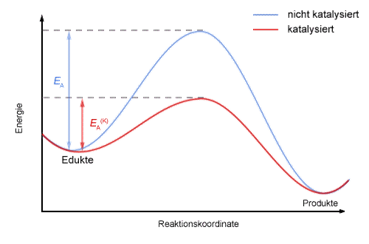
\includegraphics[width=0.9\textwidth]{Bilder/Chemie.png}
    \caption{Abgerufen von \url{http://www.chemgapedia.de/vsengine/vlu/vsc/de/ch/13/vlu/kinetik/katalyse/katalyse.vlu.html}}
    \label{fig:chemie}
\end{figure}

Es gibt im menschlichen Körper ebenfalls viele Chemische Reaktionen, welche durch Katalysatoren unterstützt werden. Diese biologischen Katalysatoren sind oftmals Enzyme welche zum Beispiel im Speichel den Prozess des Verdauens unterstützen.

Übertragen ins Psychologische kann eine chemische Reaktion als physische Handlung eines Menschen betrachtet werden. Hierbei stellt die energetische Hürde die Tatkraft eines Menschen die betroffene Handlung durchzuführen. Nudges sind als Katalysatoren zu verstehen, die in Form von positiven Nudges die Durchführung der Handlung fördern oder als negativer Nudge die Durchführung hemmen wollen. Bei einem positiven Nudge wird zum Beispiel durch das Bereitstellen von günstigeren Gegebenheiten für das Wählen der Handlung gesorgt. Dadurch sinkt die energetische Hürde und die Wahrscheinlichkeit, dass diese Handlung durchgeführt wird, ist größer.

\section{Psychologie}
\subsection{Libertärer Paternalismus}
Der Libertärer Paternalismus ist eine zugrundeliegende Philosophie des Nudgings und dient gleichzeitig als dessen Leitphilosophie. Somit sollten sich auch Unternehmen, die Nudging benutzen und das Denken der Menschen zu ihrem Vorteil beeinflussen, mir diesem Ansatz vertraut machen.
Der Begriff „Libertär“ steht für die Freiheit der Menschen und ihrer Entscheidungen. Er wird als Zusatz verwendet, um den Begriff Paternalismus so zu erweitern, dass dieser als freiheitserhaltend verstanden wird. Dies ist besonders bei einem weitreichenden und einflussreichen Konzept wie Nudging wichtig. Die Nudge-Theorie entstand mit dem Hintergrund, den Beeinflussten eine Hilfestellung bei Entscheidungen zu geben. Jedoch wird der Ansatz in der heutigen Zeit vermehrt zur Gewinnsteigerung von Konzernen, bzw. zur Verfolgung eigennütziger Ziele verwendet. Dabei betonen Thaler und Sunstein auch, dass sich Menschen einfacher und effizienter beeinflussen lassen, wenn sie Sympathie für den Einsetzenden der Nudges empfinden. Es ist demnach durchaus im Interesse der Einflussnehmenden, den Nudge unauffällig einzusetzen und im Gesamteindruck ein positives Image zu hinterlassen. Dieser Zusammenhang wird nicht direkt in dem Buch der beiden Professoren erwähnt, jedoch fügten sie im Nachhinein an, dass es einen elementaren Teil der Nudge-Theorie ausmacht \parencite{Businessballs.2013}. In dem folgenden Kapitel wird der Einsatz der Nudge-Theorie und deren Wirkung bei Menschen eingegangen. 

\subsection{The Choice Architect}
Der Begriff “Choice Architect” bezeichnet eine Führungskraft, eine Person oder eine Gruppe, welche in der Verantwortung steht, die Nudge Theorie einzusetzen.

Wie aus der Terminologie zu erkennen ist, stellt der Choice Architect die Entscheidungsmöglichkeiten des Nudges zur Auswahl. Darunter befindet sich, meistens hervorgehoben, auch die gewünschte Auswahloption. Das Ziel des Choice Architect ist es, die Mehrheit der Beeinflussten zur Wahl dieser Option zu verleiten, bzw. zu nudgen. Ein wichtiges Element des Nudging ist es, dass die finale Entscheidung von dem beeinflussten Menschen, und nicht vom Choice Architect getroffen wird. Diese Entscheidung wird in einer Mehrheit der Fälle unterbewusst getroffen. Obwohl Thaler und Sunstein nicht explizit darauf hingewiesen, dass der Choice Architect ethisch und angemessen seine Rechenschaftspflicht ausgeübt werden soll, haben beide deutlich gemacht, dass der ethische Einsatz für das Konzept des Nudgings essenziell ist.

Die Anpassung eines Nudges auf einzelne Menschen kann nicht präzise erfolgen, wenn die Zielgruppe eine größere Bevölkerungsmassen ist. Meistens entscheiden sich Choice Architects in solchen Szenarien für die Verwendung bekannter und einflussreicher Personen. So wird beispielsweise das Verhalten Dalai-Lamas eingesetzt, wenn man Meschen bei Entscheidungen über ihr Wohlbefinden beeinflussen möchte. Dies liegt vor allem daran, dass der Großteil der Menschen die Figur des Dalai-Lama mit einem gesunden Lebensstil verknüpfen. Wenn jedoch Menschen dazu bewegt werden sollen, mehr Aktivität in ihr Leben einzubauen, wird Michael B Jordan, ein bekannter amerikanischer Schauspieler, als Werbepersönlichkeit gewählt. Dieser wird von Vielen als sportliches Vorbild angesehen.

\subsection{Wie denkt der Mensch? Nutzung von Heuristiken zur Analyse}
In den ersten Seiten ihres Buches gehen Thaler und Sunstein auf die Fragen ein, warum sich Menschen wie im Vorherigen Kapitel beschreiben, beeinflussen lassen. Zudem wird dort beantwortet, warum Beeinflusste mehr auf Nudges von vertrauten Personen reagieren. Im Folgenden wird die Thematik der Entscheidungsfindung aufgearbeitet, und Rückschlüsse auf die Funktionsweise von Nudging gezogen.

Heuristiken sind das Einsatzmittel, mit dem Nudging funktioniert. In ihrer Nudge Theory haben Thaler und Sunstein fünfzehn verschiedene Arten der Heuristiken vorgestellt. Im Folgenden werden fünf davon näher betrachtet \parencite{Businessballs.2013}.

Wie auch bei der Project Theory spielt auch hier die „Loss Aversion“ eine große Rolle. Hier geht es darum, dass Menschen ein Verlust mehr trifft als einen Gewinn. Dies passiert auch, wenn der Gewinn deutlich höher ist als der Verlust. Dies ist einer der Gründe, warum Menschen dazu tendieren, auch bei hoher Gewinnchance und nur geringer Chance auf Verlust, die sicherere Variante zu nehmen. Es erscheint Vielen logischer nur einen kleinen  bis gar keinen Gewinn einzuholen, dafür aber auf das Risiko des Verlustes zu verzichten \parencite[]{Thaler.2021}.

Eine andere Heuristik ist die des „Status quo Voreingenommenheit und Trägheit“. Hier wird auf die Trägheit der Menschen eingegangen, welche Meschen dazu verleitet,  eine Situation zu akzeptieren, anstatt aktive Veränderungen vorzunehmen. Auch die Faulheit das Kleingedruckte zu lesen oder neue Arten des Lernens auszuprobieren, gehört zu dieser Heuristik. Viele Menschen kennen dieses Verhalten durch die Organspende Regel in Deutschland. Diese ist standartmäßig für jeden Deutschen so festgelegt, dass Bürger keine Organspender sind. Dies nennt sich das Opt-in-System \parencite{ApothekeAdhoc.2017}. Obwohl die Zahl der Menschen mit Bedarf auf ein Spendeorgan 12.000 beträgt, und drei Menschen pro Tag aufgrund von einem Mangel versterben \parencite{ApothekeAdhoc.2011}, ist die Quote an Menschen mit ausgefülltem Organspendeausweis unverändert niedrig. Dies liegt unteranderem daran, dass viele Deutsche nicht automatisch einen Organspendeausweis besitzen, mit dem sie bei deren Ableben als Organspender identifiziert werden können. Die meisten Personen gehen nicht den Aufwand ein, sich bewusst einen Spendeausweis zu holen, auch wenn prinzipiell eine Zustimmung zur Organspende vorhanden wäre. 

Die dritte Heuristik, welche im Rahmen dieser Arbeit beleuchtet wird, ist die Selbstkontroll-Strategie. Diese bezieht sich auf einzelne Personen, welche sich den Heuristiken bewusst sind und deshalb versuchen genau gegensätzlich zur gewünschten Reaktion zu handeln. Dies führt im Umkehrschluss zu einer eigenen Heuristik.
Im Gegensatz dazu steht der Herden-Effekt. Bei diesem hat der Mensch das Bedürfnis ein Teil eines Größeren zu sein und damit die Stärke der Masse mitzunutzen. Grundlage für das Verhalten ist die Suche nach Bestätigung von anderen. Beispiele hierfür lassen sich vor allem im Internet beobachten. Hier fühlen sich Menschen aus verschiedenen Grünen wohler als im echten Leben. Vor allem, da sie hier ein Teil einer großen Bewegung sein können, was im regionalen Umfeld den meisten nicht möglich ist.

Feedback ist die letzte, und gleichzeitig eine der wichtigsten Heuristiken. Viele Menschen kommen gerade auf der Arbeit mit der Heuristik des Feedbacks in Berührung. Beispielsweise, wenn ein Feedbackbogen ausgefüllt oder ein Mitarbeitergespräch geführt wird. Sobald die Erhebung eines Feedbacks angekündigt wird, tendieren Menschen dazu sich besser zu verhalten. Diese unbewusste Verhaltensänderung hat das Ziel, einen besseren Eindruck zu vermitteln und ein besseres Feedback zu bekommen. 
Andere Heuristiken, auf welche im Folgenden nicht näher eingegangen wird, sind Verankerung und Anpassung, Verfügbarkeit, Repräsentativität, Optimismus, Framing, Versuchung, Spotlight-Effekt, Priming, Choice Architect.

\chapter{Ist Nudging Manipulation?}

\section{Definition von Manipulation}
Unter Manipulation wird im weitesten Sinne der Versuch eines Lebewesens verstanden, das Verhalten oder die Wahrnehmung eines anderen Lebewesens zu beeinflussen oder zu ändern. \parencite[]{Horn.2019} Wenn über Manipulation geschrieben wird, ist dies meist positiv oder negativ konnotiert. Dies dient der Differenzierung von missbräuchlicher gegenüber weniger schwerwiegender Manipulation. Unter Letzteres fällt beispielsweise die Überredung. Thaler und Sunstein plädierten durchwegs für eine ethische Nutzung von Nudging. Ob dies eingehalten wird kommt auf den Choice Architect und auf die Absicht hinter dem Nudge an. 

\section{Differenzierung von Nudging und Manipulation}
Beim Nudging handelt es sich laut Thaler und Sunstein nicht um Manipulation. Dies machen sie durch ihre starke Distanzierung ihrer Theorie von manipulativer Nutzung. Dies fängt schon mit ihrer Leitphilosophie Libertärer Paternalismus an. Hier setzen sie wohl weislich „Libertärer“ also „Autonom“ davor. Doch immer wieder kommt die Debatte auf, dass es sich bei Nudging um Manipulation handelt. Wenn zum Beispiel in Kalifornien die Regierung durchsetzt, dass Nachbarn gegenseitig ihren Stromverbrauch gezeigt wird hat dies das Ziel, den Verbrauch zu senken. Das ist noch nicht als klare Manipulation erkennbar, sondern kann als ein Nudge in Richtung umweltbewusstes Verhalten gesehen werden. Argumente für die Klassifizierung als Nudge sind die Freiwilligkeit, da Haushalte mehr Strom verbrauchen können, wenn gewollt. Andererseits kann man es als soziale Manipulation ansehen, da ein hoher Verbrauch von den Nachbarn, und daher vom gesellschaftlichen Umfeld, verurteilt wird. \parencite{BerufsverbandDeutscherPsychologinnenundPsychologen.2015}. 
Ein anderes Beispiel, welches viele Männer in Urinalen schon miterlebt haben, ist das der Plastikfliege im Urinal. Die meisten Männer versuchen hier die Fliege zu treffen, weshalb 80\% weniger Urin daneben geht auf öffentlichen Toiletten. Dies ist generell nicht als Manipulation angesehen zu werden, müsste der Einfluss unterbewusst stattfinden. Zudem ist der Einsatz solcher Hilfen gerechtfertigt, da eine saubere Toilette im Interesse der Öffentlichkeit ist \parencite{Brautzsch.2020}.
Um über die zukünftige Nutzung von Nudging zu entscheiden, müssen klare Unterschiede zu eigennütziger Motivation definiert und eingehalten werden. Aktuell sind die formalen Grenzen zwischen diesen allerdings noch sehr verschwommen.
Bei der Verwendung von Nudging im kommerziellen Umfeld ist es wichtig, dass Choice Architects nicht mit der Intention der Manipulation handeln und diese als Nudging tarnen. Stattdessen sollte das Nudging stets mit der Absicht verwendet werden, das Wohl der Kunden und ihre Erfahrung positiv zu beeinflussen. Wird Nudging mit eigennützigen oder primär profitorientierten Intentionen verwendet, fällt es ebenfalls in den Bereich der Manipulation.
Ob Nudging unter Manipulation läuft, wird wahrscheinlich für das Bestehen des Nudgings eine umstrittene Frage sein, auf die viele mit Ja und andere mit Nein antworten. 
Das Wichtigste ist, dass wenn Nudging verwendet wird, der Choice Architect nicht mit der Intention der Manipulation, sondern mit der Intention der Entscheidung Hilfe zum Wohl des anderen handelt. Denn Nudging kann als Manipulation verwendet werden, wenn mit Bösen Absichten gehandelt wird.

\chapter{Digital Nudging}
\section{Definition von Digital Nudging}
Jeden Tag trifft ein Mensch durchschnittlich 10.000 Entscheidungen, manche größer, mache kleiner. In der heutigen Zeit, in der eine Welt ohne Technology und Digitalisierung nicht mehr vorstellbar wäre, werden viele dieser Entscheidungen online und somit digital getroffen. Weshalb es keinesfalls verwunderlich ist, dass nudging auch im digitalen Raum verwendet wird. Das sogenannte Digital nudging. Digitales Nudging ist die Verwendung von Elementen der Benutzeroberfläche, um das Verhalten der Menschen in digitalen Entscheidungsumgebungen zu steuern \parencite[]{Weinmann.2016}. Hier liegt der Focus auf dem Design der Benutzeroberfläche. Typische Nudges können hier Mitteilungen sein, die einen an Produkte im Warenkorb erinnern, die noch gekauft werden sollen. Oder ein Fehler, der schon vorhersehbar ist und deshalb verhindert werden soll. Ein Beispiel, dass jeder Erwachsene kennt, ist hier, dass der Geldautomat nur dann das Geld ausgibt, wenn die Karte von Besitzer schon entnommen wurde.
Digital Nudges sollten auch im digitalen Umfeld als eine Hilfestellung dienen, damit Nutzer basieren darauf die für sie Beste Entscheidung treffen können. 
Möglichkeiten, um Nudges hervorzuheben sind grafische Designanpassungen. Dies kann durch Text und Farbe erreicht werden. Anordnungen von Inhalten, sowie auch durch kleine Animation, damit die Aufmerksamkeit auf die Digital Nudges gelenkt wird.

\section{Ethische Grundlagen}
Die Betrachtung der ethischen Grundlagen bildet das Fundament für die Diskussion über Nutzen, Chancen und Risiken von Digital Nudging, vor allem im ökonomischen Umfeld. Zudem ist sie notwendig, um einen Nudge von einer Manipulation bzw. Überredung des Users abzugrenzen \parencite[S. 3]{Jesse.2021}. Das ethische Fundament von Nudging ist nicht exklusiv für den digitalen Rahmen anzuwenden, jedoch ist die Einhaltung hier wichtiger.

Laut Kahnemann spricht die Nutzung von mobilen Anwendungen bei einem Großteil der Bevölkerung das intuitive Denksystem, auch System 1 genannt, an. Dies steht im Gegensatz zum rationalen und überdenkenden System 2, welches Viele bei Kaufentscheidungen im Laden nutzen. Durch die vorherrschende Nutzung von System 1 handeln Personen im digitalen Umfeld impulsiver und mit weniger Überdenkzeit, \parencite[Absatz 1b]{Kahneman.2012} was die Wirksamkeit von Nudges erheblich steigert. Zudem vereinfachen die Einsatzmöglichkeiten von Algorithmen und die schnelle Anpassungsfähigkeit von User Interfaces die Individualisierung von Nudges, sowie das Testen deren Wirksamkeit \parencite[S. 88]{Reisch.2020}. So teilt Instagram beispielsweise ihre User in zwei Gruppen auf, um Interface-Änderungen zu testen. Bei einer Hälfte wird das Update ausgespiel, die andere Hälfte bleibt auf der bereits eingesetzten Software-Version. Damit ist es Instagram möglich, einen direkten Vergleich zwischen beiden Oberflächen zu haben, und Rückschlüsse mit minimaler Verzerrung zu ziehen.
\subsection{Autonomität}
Die wesentliche ethische Grundlage ist die Gewährleistung von Autonomität des Users bei der Konfrontation mit einem Nudge. Das bedeutet, dass die uneingeschränkte Wahlfreiheit des Nutzenden zwischen allen Optionen gewährleistet werden muss. \parencite[S. 88]{Reisch.2020} Jedoch ist die freie Wahl nicht nur auf die Verfügbarkeit aller Optionen zu beziehen, sondern die Entscheidung des Nutzenden sollte bedacht, und ohne erheblichen Einfluss von Dritten getroffen werden. \parencite[S. 6]{Lembcke.2019}

Ein solche Ausgangssituation ohne externe Einflüsse ist oft nicht komplett vermeidbar, da diese nicht von der Plattform beeinflusst werden können. Jedoch sollten die Einflüsse innerhalb der Anwendung auf ein Minimum reduziert werden. \parencite[S. 88]{Reisch.2020}Wenn man im Browser nach Hilfsmitteln gegen Kopfschmerzen sucht, bekommt man häufig Websites von bekannten Marken vorgeschlagen. Diese informieren meist zuerst über die Ursachen von Kopfschmerzen, und geben danach Tipps zur Linderung der Symptome, welche die Produkte der Marke bewerben. Aus eingener Nachforschung lässt sich erkennen, dass Nutzende dadurch zum Kauf bewegt werden, ohne Alternativen abzuwägen. Dies ist aus Sicht der Marke sinnvoll, schränkt allerdings in gewisser Weise die Autonomität des Users ein. Zwar gibt es keine Auswahl an verschiedenen Anbietern, jedoch steht es dem Besuchenden der Website frei, ob er das Produkt tatsächlich kaufen möchte.

Wenn bei der Betrachtung eines Nudges die Autonomität nicht eindeutig festzustellen ist, bzw. diese von der Perspektive abhängig ist, kann die ethische Fundierung anhand der anderen Grundlagen bestimmt werden.
\subsection{Transparenz}
Die Transparenz eines Nudges ist gegeben, wenn die benutzende Person den Einfluss durch den Nudge, sowie die Ziele des Nudges, erkennt. Zudem sollten alle Optionen sichtbar und als Solche zu erkennen, sowie die Bedeutung dieser Optionen klar verständlich sein. \parencite[S. 89]{Reisch.2020} Dadurch steht die Transparenz im direkten Zusammenhang mit der Autonomität des Nudges. Wenn eine Auswahl an Optionen besteht, diese allerdings nicht klar sichtbar sind, ist die Transparenz nicht sichergestellt, und somit durch mangelnde Auswahl auch die Autonomität eingeschränkt.
\subsection{Zielrechtfertigung}
Nudges können, je nach Ort und Art des Einsatzes, verschiedene Ziele verfolgen. Um ethisch korrekt zu sein, müssen soziale oder nutzerbezogene Ziele verfolgt werden. Eigennützige Ziele aus Sicht des Providers sind selten ethisch zu rechtfertigen, außer es ist nachweisbar, dass die Ziele mit denen eines Großteils der Nutzenden übereinstimmen. Im Gegensatz dazu, können soziale Ziele sogar dann ethisch korrekt sein, wenn Nutzende ihnen nicht zustimmen, solange kein Beeinflusster den Einfluss als einschränkend oder untragbar ansieht. \parencite[S. 89]{Reisch.2020}\parencite[S. 7]{Lembcke.2019} In diese Kategorie fallen vor allem Self-Nudges, die den Nutzenden zu einem besseren Verhalten bewegen, wie zum Beispiel Aufforderungen für Spenden. Auch die von Google Maps vorgeschlagene Option, den kraftstoffsparendsten und damit umweltfreundlichsten Weg für die Autofahrt anzuzeigen, kann als diese Art von Nudge kategorisiert werden.
\chapter{Beispiele für Digital Nudges}
\section{IKEA: Positives Vorbild im E-Commerce}
\subsection{Einführung in das Beispiel und Problemstellung}
Vor allem im Bereich Wohnen ist Kunden eine große Auswahl wichtig. Es erlaubt sowohl Individualisierung bei der Gestaltung eines Wohnraumes, als auch Anpassung an das vorhandene Budget. Dadurch wird die Zielgruppe vergrößert und mehr Umsatz generiert. Bei einer zu großen Auswahl an Optionen wird häufig ein umgekehrtes Phänomen beobachtet, dem Choice Overload Effect, zu Deutsch das Auswahlparadoxon. \parencite[S. 58]{Bauer.2018}

Dieses beschreibt die Tendenz von Kaufenden, eine große Auswahl zu favorisieren, zu einer Kaufentscheidung kommt es allerdings häufiger, wenn weniger Optionen zur Verfügung stehen. Das liegt daran, dass potenzielle Kunden den Überblick verlieren und sich überfordert fühlen. \parencite[S. 58]{Bauer.2018}Die Konsequenz ist oft die Aufschiebung der Entscheidung, der Wechsel zur Konkurrenz mit weniger Auswahl. Eine andere Möglichkeit, vor allem im digitalen Umfeld, ist die spontane Entscheidung für ein Produkt. Erst nach dem Kauf werden die Details näher betrachtet, und möglicherweise festgestellt, dass das Produkt nicht den Wünschen und Anforderungen entspricht.

Vor diesem Problem steht auch die Firma IKEA. Laut ihrer Website gibt es allein für die Kategorie Betten 2410 Modelle mit verschiedenen Ausführungen

und Kombinationen.\parencite{InterIKEASystemsB.V..2022} Dieses Produktportfolio ist wichtig für IKEA, um mit den verschiedenen Preiskategorien und Designlinien möglichst viele Kunden anzusprechen. Allerdings sind selbst nach der Auswahl von Filtern noch bis zu hundert verschiedene Optionen verfügbar. Diese unterscheiden sich meist nur in kleinen Details. Um den Kunden den Vergleich ihrer Auswahl zu vereinfachen, setzt IKEA Digital Nudging ein.
\subsection{Aufbau und Wirkung}
\begin{figure}[ht]
    \centering
    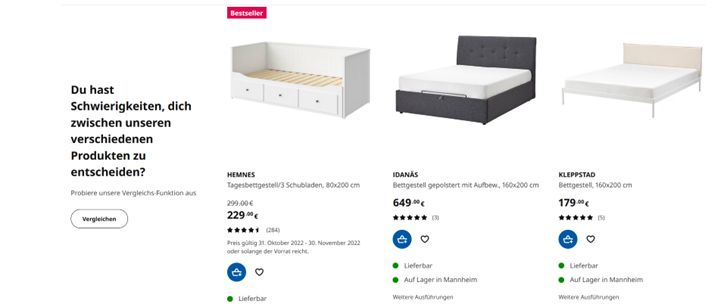
\includegraphics[width=0.9\textwidth]{Bilder/Ikea_Nudge.png}
    \caption{Nudge zum Nutzen der Vergleichsfunktion auf \url{https://www.ikea.de} in der Produktsuche}
    \label{fig:Ikea-Nudge}
\end{figure}
In der zweiten Reihe der angezeigten Optionen nutzt IKEA die linke Spalte, um den Nutzenden auf die Vergleichen-Funktion hinzuweisen. Der Hinweis ist so angebracht, dass er für Nutzende, die das vorhandene Angebot überfliegen möchten, nicht störend ist. Dennoch ist er auffällig genug, um wahrgenommen zu werden. Im Fokus steht vor allem der deutlich größere Schriftzug, welcher die Probleme des Nutzenden anspricht. Direkt darunter wird die Vergleichen-Funktion als Lösung aufgezeigt.

\subsection{Bewertung anhand der ethischen Grundlagen}
Der Nudge ermöglicht Nutzenden die freie Entschidung, ob die Vergleichen-Funktion genutzt wird. Es wird auch nicht aktiv von der Website versucht, den User zur Verwendung der Funktion zu überzeugen. Der Nudge ermöglicht dem Kaufenden eine bessere Entscheidung bezogen auf den Kauf des Produktes. Dadurch bleibt die Autonomität des Nutzenden bestehen, und wird bei der Kaufentscheidung zusätzlich verstärkt.

Auch sind die Auswahlfelder klar erkennbar, und verleiten den User nicht dazu, Optionen auszuwählen die er nicht versteht bzw. nicht auswählen wollte. Die Benennung ist klar verständlich und nicht umzudeuten. Hinter dem Button sind auch nicht zusätzliche Funktionen oder Aktionen versteckt, die der Nutzende eigentlich nicht auswählen wollte. Auch verzichtet IKEA auf Voreinstellungen und erlaubt es dem User seine Suche individuell anzupassen. Diese Punkte sprechen für eine hohe Transparenz des Nudges, was die zweite ethische Grundlage erfüllt.

Bei der Zielrechtfertigung ist IKEA darauf fokussiert, die User Experience für interessierte Personen zu verbessern, und diese dadurch eher zum Kauf zu bewegen. Das bringt zwar positive Aspekte für IKEA, jedoch ist das Hauptziel des Nudges, den Besuch der Website für Kunden möglichst angenehm zu gestalten.

\section{Cookie Banner: Manipulativ?}
\subsection{Einführung in das Beispiel und Problemstellung}
Internetseiten nutzen zum Anzeigen und Senden von Daten das sogenannte \ac{HTTP}. Bei \ac{HTTP} handelt es sich um ein sogenanntes ``stateless'' (zustandsloses) Protokoll, d.h. alle Anfragen und Transaktionen zwischen dem Nutzer und der aufgerufenen Internetseite sind unabhängig voneinander. Dadurch fällt es schwer, Zusammenhänge und Nutzerdaten mehrerer Anfragen mitzusenden und abrufbar zu halten.

Cookies werden eingesetzt, wenn bestimmte Infos zwischen mehreren Anfragen gespeichert werden sollen. Sie sind kleine Dateien, welche von der aufzurufenden Internetseite angefordert und gesendet werden. Die Cookies werden dann vom genutzten Internetbrowser angelegt und verwaltet. Sie sind dabei immer spezisich für die Seite, die sie anfragt und sendet und werden genutzt, um beispielsweise Internetseiten mit Kontofunktionen zu realisieren. \parencite[S. 4-6]{Kristol.}

Obwohl Cookies spezifisch für jede Internetseite sind und ein Verknüpfen von Nutzerdaten über mehrere Internetseiten hinweg nicht möglich sein sollte, wurde durch die Funktionsweise des Internets schnell eine Möglichkeit gefunden, Cookies für mehrere Seiten zu nutzen.

Dabei wird neben der gewünschten Internetseite noch eine weitere Seite geladen, welche den Cookie setzt und anfordert. Wenn dieses System über mehrere Internetseiten hinweg genutzt wird, können die Interessen eines Nutzers nachverfolgt werden. Man spricht hierbei vom ``Third Party Cookies'', da das Datensammeln nicht direkt durch den Seitenbetreiber selbst passiert. \parencite[S. 2608]{Bielova.2017}

\begin{figure}[ht]
	\centering
	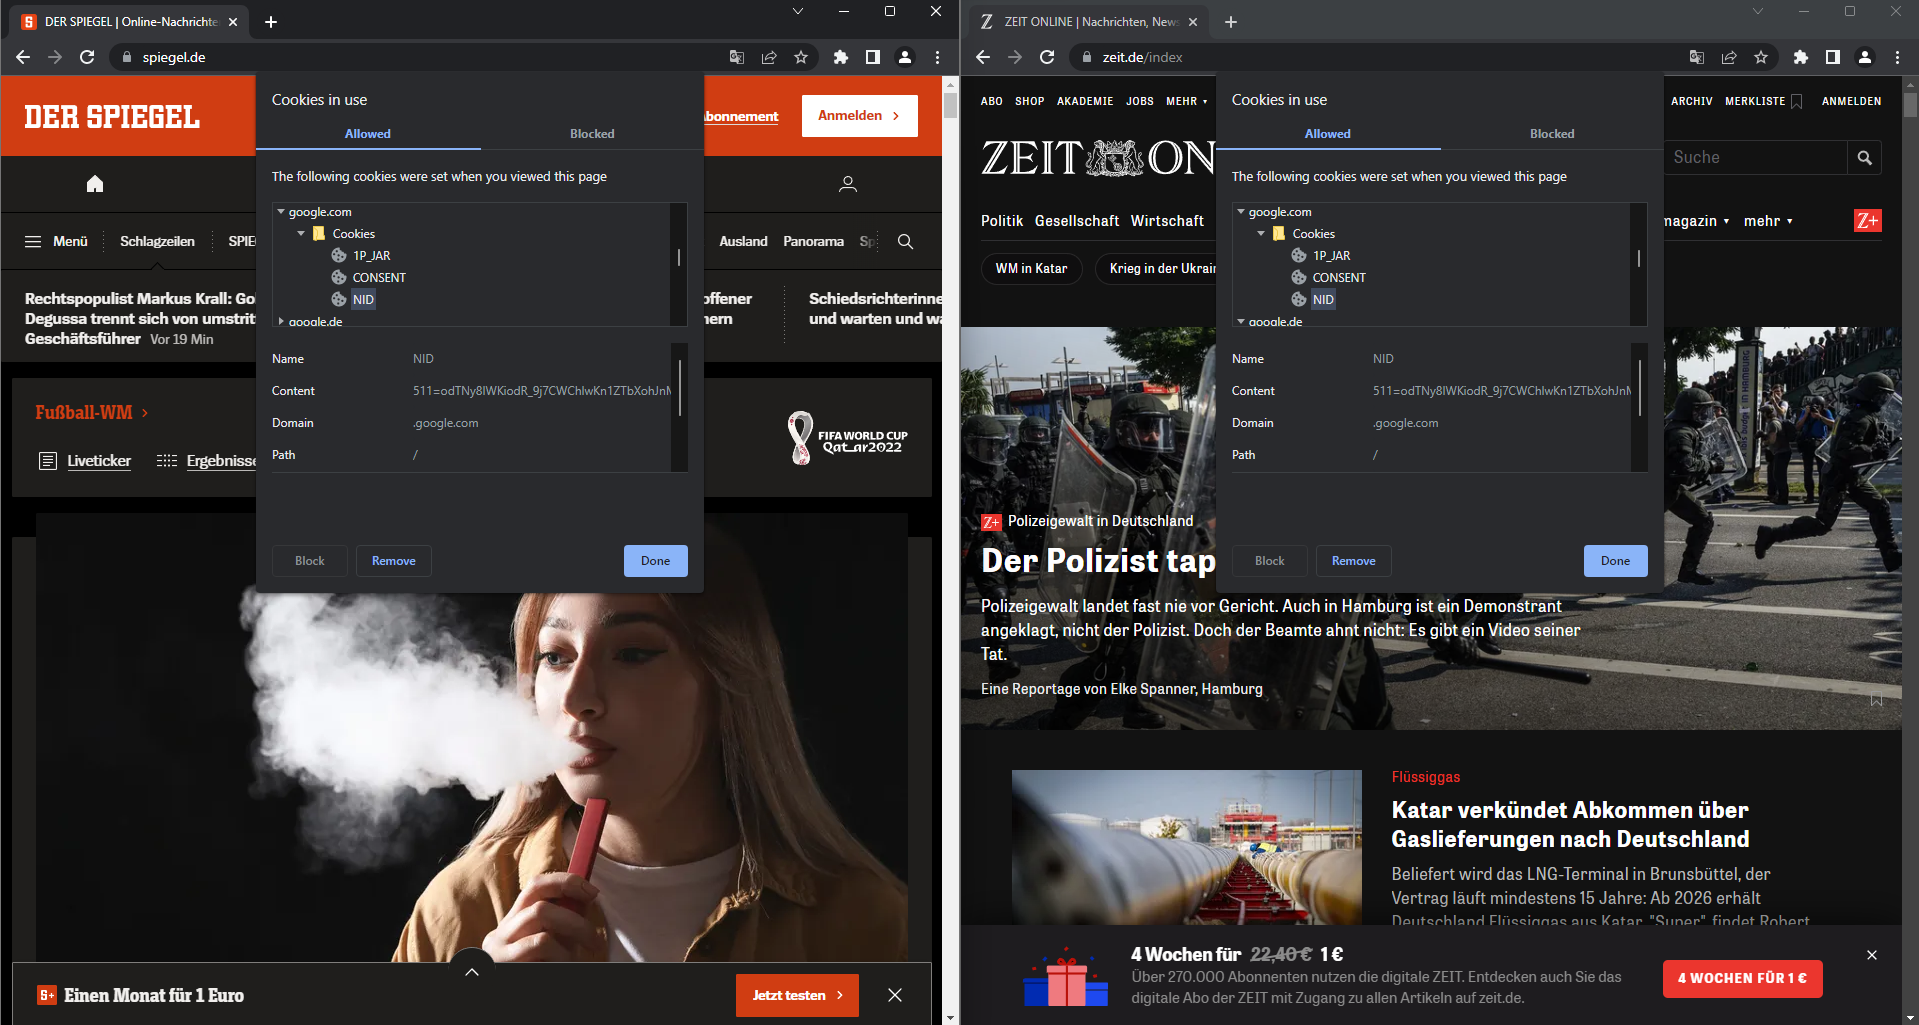
\includegraphics[width=1\textwidth]{Bilder/Cookies.png} 
	\caption{Ein Third Party Cookie von Google, welcher bei \url{https://www.spiegel.de} und \url{https://www.zeit.de} genutzt wird}
	\label{fig:Third-Party}
\end{figure}

Die \ac{EU} hat 2016 die \ac{DSGVO} verabschiedet. \parencite{EuropaischeUnion.2016} Seitdem gibt es für Cookies in der \ac{EU} einen rechtlichen Rahmen zur Verwendung jener. Dieser sieht vor, dass lediglich ``First Party Cookies'', also Cookies, welche direkt von der aufgerufenen Internetseite erstellt werden, genutzt werden dürfen. Entsprechenden ``Third Party Cookies'', welche hauptsächlich zum Sammeln von Nutzerdaten genutzt werden, muss der Nutzer nach der \ac{DSGVO} erst explizit zustimmen. Die \ac{EU} erhofft sich davon mehr Transparenz im Bezug auf die Verarbeitung personenbezogener Daten. \parencite[S. 84]{EuropaischeUnion.2016}

Unternehmen ist in vielen Fällen jedoch daran gelegen, möglichst viele ``Third Party Cookies'' einzubinden. So gibt es ganze Geschäftsmodelle, welche Cookies zu Werbe- und Analysezwecken nutzen und durch das effektive Sammeln und Auswerten von Daten Umsatz generieren.\parencite[S. 418-420]{.2012} Durch die gegebenen Umstände entwickelte sich so der Trend, dass zur Einwilligung in die Datensammlung ein Nudge genutzt wird, welcher die Entscheidung beeinflussen soll.

\subsection{Aufbau und Wirkung}
Die Zustimmung zu Cookies wird auf Internetseiten meist in Form eines Banners realisiert, welcher den Nudge enthält. Der Cookie Banner fragt dabei den Nutzer, ob das Einsetzen von Drittanbieter Cookies und damit das Sammeln von Daten gestattet ist. Die Gestaltung weicht dabei je nach Plattform stark voneinander ab.

\begin{figure}[ht]
    \centering
    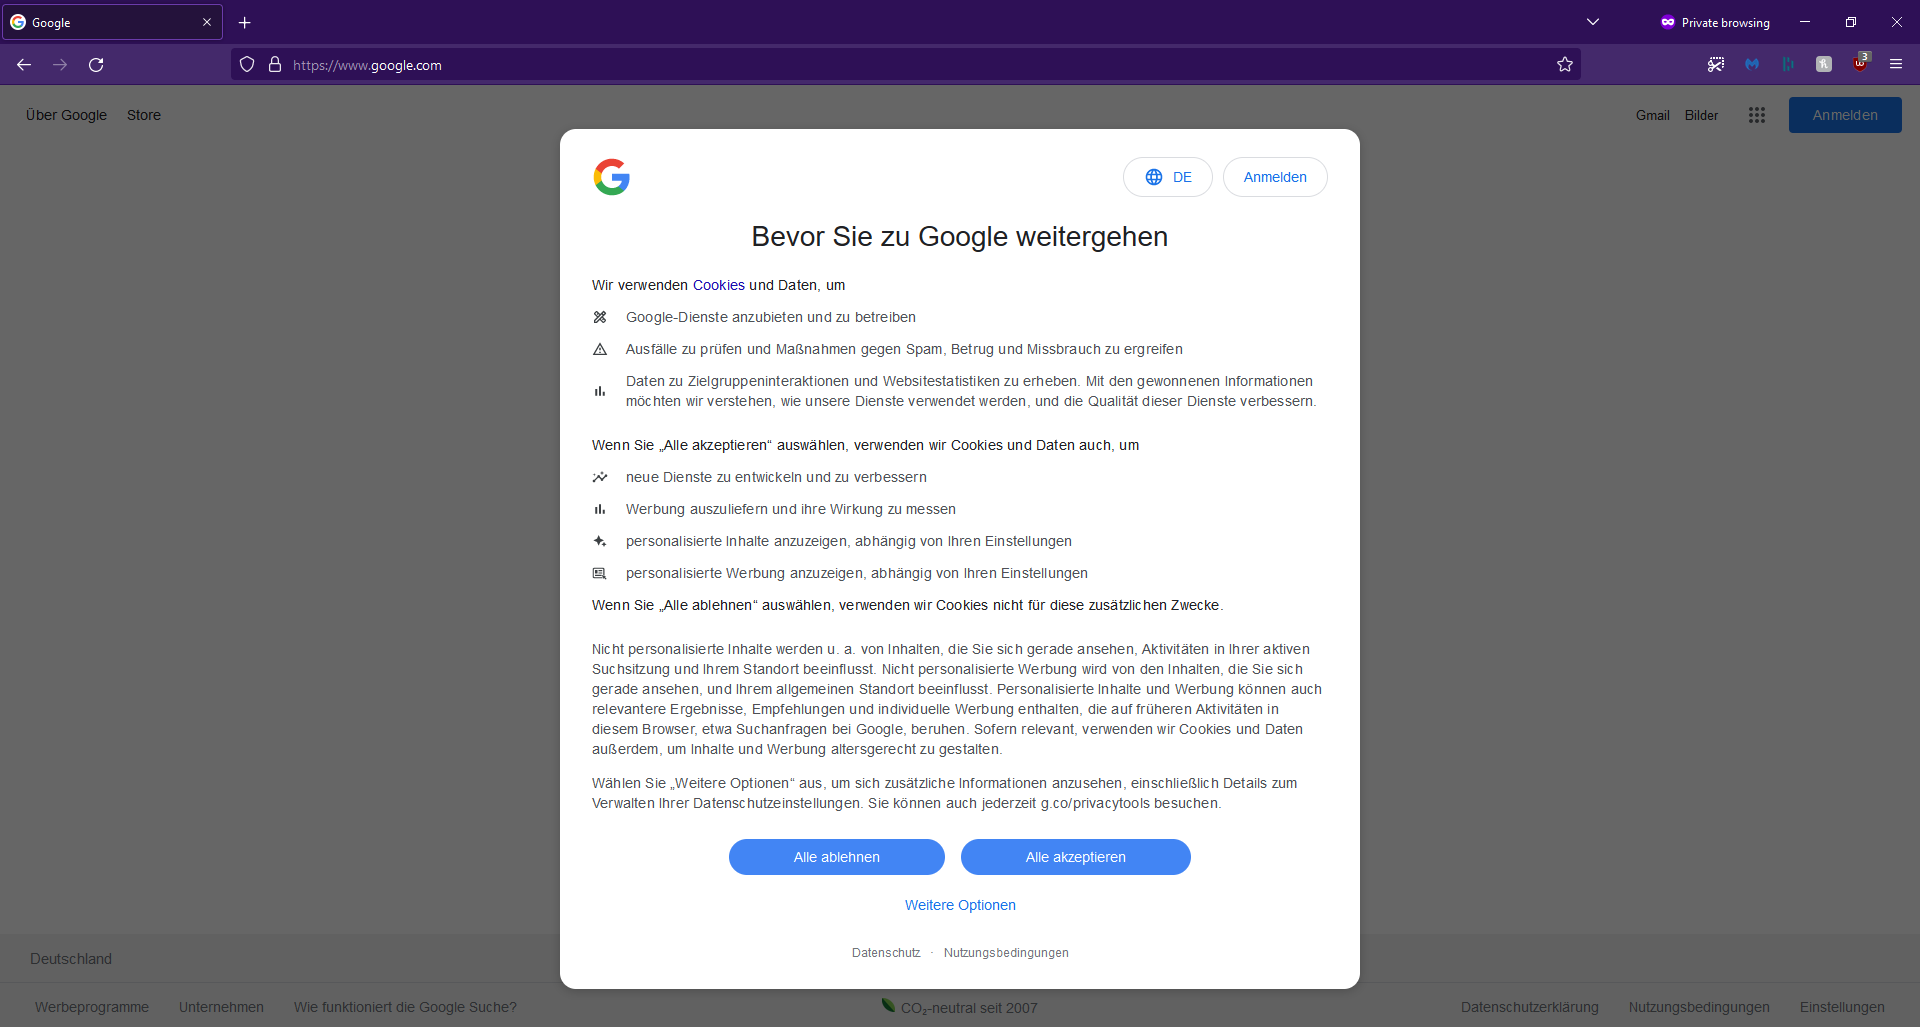
\includegraphics[width=1\textwidth]{Bilder/Google_Banner.png}
    \caption{Cookie Banner auf \url{https://www.google.com}}
    \label{fig:Google-Cookie}
\end{figure}

Beim ersten Aufrufen der Website \url{https://www.google.com} wird der Cookiebanner angezeigt. Dabei wird bereits direkt ein Nudge auffällig. Der Banner wird zentral über dem eigentlichen Inhalt des Bildschirms platziert. Der Nutzer, welcher gerade etwas bei Google suchen möchte, muss daher zuerst mit dem Banner interagieren. Google bietet hier einen Knopf ``Alles Akzeptieren'' und ``Alles ablehnen'' an. Dennoch wird hier bereits Einfluss auf den Nutzer genommen, da sein Nutzungserlebnis direkt gestört wird und er erst einen der beiden Knöpfe drücken muss, um mit seiner Arbeit fortzufahren.

Auf der Webseite von Facebook (\url{https://www.facebook.com/de}) wird neben dem inhaltsverdeckenden Banner ein weiterer Nudge eingesetzt. Die Option ``Erforderliche und optionale Cookies erlauben'' ist in einem auffälligen Blau markiert, während die Option ``Nur erforderliche Cookies erlauben'' in einer grauen Farbe gezeigt wird.

\begin{figure}[ht]
    \centering
    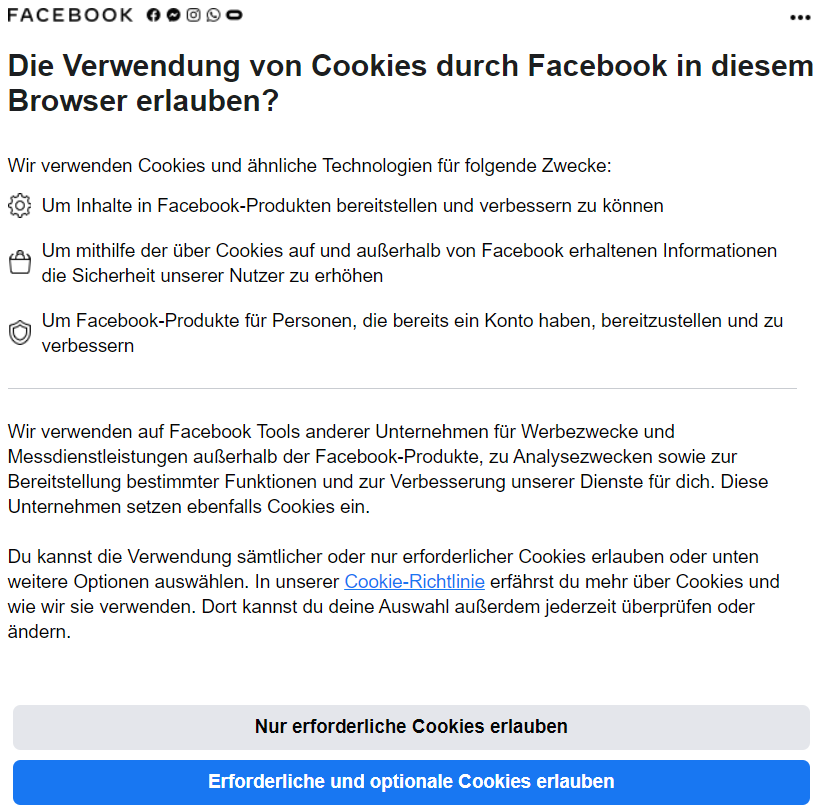
\includegraphics[width=0.8\textwidth]{Bilder/Facebook_Banner.png}
    \caption{Cookie Banner auf \url{https://www.facebook.com/de} mit farblich unterschiedlichen Knöpfen}
    \label{fig:Facebook-Cookie}
\end{figure}

Die farbliche Hervorhebung einer Option erscheint für den Nutzer hierbei wie eine Empfehlung und sticht mehr ins Auge, als der hellgraue Farbton, welcher sehr ähnlich zum Hintergrund wirkt. Hervorhebung einer gewünschten Option kann nicht nur durch Farbe, sondern auch durch Positionierung und Größe innerhalb des Banners passieren.

Eine weitere Möglichkeit, den Nutzer in seiner Entscheidung zu beeinflussen, stellt das Verlagern der Ablehnen Funktion auf eine Extra Seite dar. Hierbei wird dem Nutzer lediglich eine Option zum Akzeptieren und eine Option zum Ansehen diverser Einstellungen bezüglich des Datenschutzes angeboten.

\begin{figure}[ht]
    \centering
    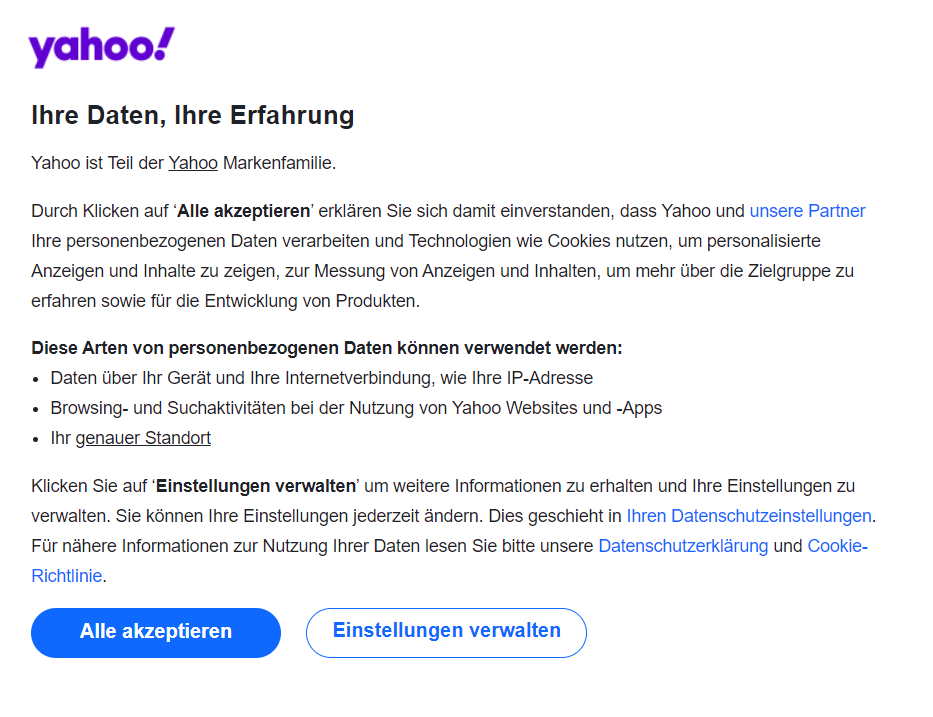
\includegraphics[width=0.8\textwidth]{Bilder/Yahoo_Banner.png}
    \caption{Cookie Banner auf \url{https://www.yahoo.de} mit Einstellungsknopf}
    \label{fig:Yahoo-Cookie}
\end{figure}

Dieses Verlagern der Ablehnenfunktion auf eine weitere Seite ist besonders effektiv, wenn der Nudge dazu genutzt werden soll, dass Nutzer tendenziell dem Datensammeln zustimmen. Die Zustimmung aller Cookies ist 22 - 23 \% wahrscheinlicher, wenn die Ablehnenfunktion nicht direkt im Banner enthalten ist. \parencite[S. 8]{Nouwens.2020}

\subsection{Bewertung anhand der ethischen Grundlagen}

Je nach Funktionsweise lässt sich nachweisen, dass die hier gezeigten Beispiele gegen die in Kapitel HIER EINSETZEN verstoßen.
Während die Einblendung von Google (siehe Abbildung \ref{fig:Google-Cookie}) mit den Optionen ``Alles Akzeptieren'' und ``Alles ablehnen'' eine transparente und autonome Auswahl der Einstellungen ermöglicht, lässt sich argumentieren, dass die Banner von Facebook (siehe Abbildung \ref{fig:Facebook-Cookie}) und Yahoo (siehe \ref{fig:Yahoo-Cookie}) gegen ethische Grundsätze von digitalen Nudges verstoßen.

In beiden Fällen ist die Transparenz eingeschränkt, da eine Option (Alles akzeptieren) farblich hervorgehoben ist und die Wahl damit nicht mehr neutral ist. Yahoo geht außerdem einen Schritt weiter und bietet gar nicht mehr alle Optionen direkt an (``Alles ablehnen''), sondern versteckt den Inhalt auf einer Einstellungsseite, was nicht nur Transparenz sondern auch Autonomie einschränkt.

Deutsche Zeitungsanbieter nutzen dieses Prinzip und bieten keine Option zum Ablehnen mehr an. Hier wird lediglich vorgeschlagen, die Cookierichtlinien zu akzeptieren oder für ein cookiefreies Modell zu bezahlen.

\begin{figure}
    \centering
    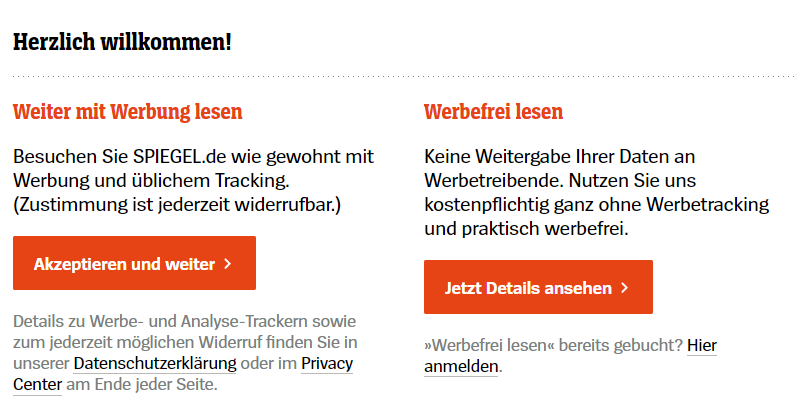
\includegraphics[width=0.9\textwidth]{Bilder/Spiegel_Banner.png}
    \caption{Cookie Banner auf \url{https://www.spiegel.de} mit Bezahlfunktion}
    \label{fig:Spiegel-Cookie}
\end{figure}

Hier sind Autonomität und Transparenz noch eingeschränkter, da gar nicht mehr alle Optionen (Cookies ablehnen) angeboten werden. Dem Nutzer wird lediglich angeboten, alle Cookies zu akzeptieren, eine Option alles abzulehnen gibt es nicht mehr.

Abschließend lässt sich sagen, dass die Nutzung von Cookie Bannern bei bekannten Plattformen klar gegen ethische Grundlagen verstößt. Neben den Idealen der Autonomität und Transparenz, verstoßen alle genannten Beispiele auch gegen den Grundsatz der Zielrechtfertigung, da mit dem Aktivieren der Cookies weder soziale noch nutzerfreundliche und lediglich Interessen der Plattform verfolgt werden. Auch rechtlich sind die gezeigten Beispiele bereits kritisiert worden. So verurteilte die französische Datenschutzbehörde Facebook und Google zu hohen Geldstrafen aufgrund von Verstößen gegen die DSGVO im Bezug auf die Implementierung von Cookie-Bannern. \parencite{AnnaBiselli.2022}
\chapter{Ethische und rechtliche Probleme bei Digital Nudging}
Dieses Kapitel diskutiert Risiken und Probleme, die bei der Verwendung von Digital Nudging auftreten können.
\section{Helles und dunkles Nudging}
Bei der Nutzung von Nudges im digitalen Bereich lässt sich grundsätzlich zwischen hellem und dunklem Nudging unterschieden. Dabei beschreibt helles Nudging einen nach den ethischen Grundlagen "guten" Zweck, während dunkles (dark) Nudging für Zwecke steht, die gegen die ethischen Grundlagen verstoßen.

Wichtig ist dabei, dass Nudging als Instrument in der Diskussion erst einmal neutral ist. Erst durch die Definition eines Anwendungsfalls kann darüber diskutiert werden, ob es sich um einen hellen oder dunklen Nudge handelt.

Dennoch lässt sich in der Wirtschaft abzeichnen, dass Nudging zunehmend für unethische Zwecke verwendet wird. Dafür haben sich die Begriffe ``Dark Nudging'', ``Sludges'' und ``Dark Patterns'' etabliert. \parencite[S. 73-74]{Narayanan.2020} Der Begriff Dark Patterns wurde dabei 2010 erstmals von  Brignull definiert und beschreibt Tricks in Webseiten und Apps, die Nutzer:Innen zu Handlungen bewegen, die von ihrer eigentlich gewünschten Handlung abweisen. \parencite{Brignull.2010}

Wissenschaftler haben herausgefunden, dass Dark Patterns in über 1200 Shopping Seiten \parencite[S. 2]{Mathur.2019} und in mehr als 95\% von beliebten Android Apps \parencite[S. 5]{DiGeronimo.2020} implementiert sind. Daran lässt sich erkennen, dass Dark Nudging sehr in den Alltag von Nutzerinnen und Nutzern eingreift und kein Randphänomen ist.

Thaler, der wie in Kapitel (HIER EINSETZEN) die Theorie hinter Nudging eingeführt hat, distanziert sich mittlerweile öffentlich von der Dark Patterns Nutzung seiner Idee. Er nennt unethische Nudges ``Sludges''. Seiner Ansicht nach sollten Nudges nur genutzt werden, um die Umgebung, in der Menschen Enrscheidungen treffen angenehmer zu gestalten. Dies ermögliche selbstbewusstere Entscheidungen. Dark Pattern beschreibt er als "nudging for evil". \parencite{Thaler.2018}

\section{Rechtliche Situation}
Die Präsenz des Themas im alltäglichen Gebrauch lässt auch die Gesetzgebung in Deutschland und der \ac{EU} auf das Thema aufmerksam werden. Auch wenn es bisher keine einheitliche Regelung bezüglich Digital Nudging und Dark Patterns gibt, so sind in Einzelfällen (wie bspw. in HIER KAPITEL EINSETZEN) bereits rechtliche Grundlagen zur Nutzung von Nudges gesetzt worden.

Der Gewinnspielbetreiber "Planet49" hatte bei seinem Cookie Banner standardmäßig alle Cookies mit Ankreuzkästchen aktiviert. Zum Ablehnen der Datensammlung war es notwendig, die Häkchen nach und nach anzuklicken. Der Bundesverband der deutschen Verbraucherzentralen und Verbraucherverbände hat gegen diese Implementierung geklagt. In einem Urteil des \ac{EuGH}, welches später durch den deutschen \ac{BGH} bestätigt wurde, wird erläutert, dass eine wirksame Einwilligung nicht durch vorausgewählte Einstellungen erfolgen könne. Außerdem seien zu einer vollständigen Einwilligung weitere Informationen notwendig, wie z.B. die Funktionsdauer der Cookies oder mit welchen Drittanbietern sie geteilt werden. \parencite{Hartung.2020}

Aktuell befasst sich die \ac{EU} im Rahmen des \ac{DSA} mit Dark Patterns. So plant die \ac{EU}, Dark Patterns weitreichend zu verbieten. ``Anbietern von Online-Plattformen sollte es [...] untersagt sein, die Nutzer in die Irre zu führen oder zu etwas zu verleiten und die Autonomie, die Entscheidungsfreiheit oder die Auswahlmöglichkeiten der Nutzer durch den Aufbau, die Gestaltung oder die Funktionen einer Online-Schnittstelle oder eines Teils davon zu verzerren oder zu beeinträchtigen.'' \parencite[S. 18]{EuropaischeUnion.2022} Damit gibt es erstmalig eine Rechtsgrundlage zur allgemeinen Benutzung von Nudes im digitalen Raum. Dennoch gibt es Bedenken, dass die Forderungen des \ac{DSA} nicht weitreichend genug seinen, etwa weil sich der die Regelungen nur auf ``Online-Plattformen'' beziehen, worunter nicht alle Internetseiten fallen. \parencite{King.2022} Es bleibt abzuwarten, wie effektiv die Regelungen des \ac{DSA} sind und ob Plattformbetreiber ihre Inhalte nach Inkrafttreten der Verordnung in den Mitgliedsstaaten anpassen.
\chapter{Fazit}
Wie in den vorausgegangenen Kapiteln erarbeitet, ist Digital Nudging und seine Wirkung stark davon abhängig, wie und wer es einsetzt. Als Hilfestellung im e-commerce bietet Digital Nudging Vorteile für Kunden, und damit einhergehend einen höheren Profit für das Unternehmen. Nudges können als Self-Nudges Angewohnheiten und Verhalten von Nutzenden verbessern, bei Spendenportalen die Quote an Spendenden erhöhen und oder durch Standardeinstellungen bei z.B. Google Maps Personen dazu bewegen, umweltfreundlicher zu fahren.

Wenn die ethischen Grundsätze jedoch missachtet werden, tritt schnell Unzufriedenheit bei den Kunden auf, und ein negatives Bild gegenüber dem Unternehmen entsteht. Es ist zwar möglich, durch Cookie-Banner oder auch Voreinstellungen zum Abonnieren von Newslettern bei der Bezahlung kurzfristig mehr Gewinn zu generieren, jedoch entwickeln Kunden unterbewusst eine Abneigung gegen das Unternehmen, welche dem langfristigen Unternehmenserfolg schaden können.

Aus Interesse an einer freien Entscheidungsbasis ist eine Überarbeitung der Gesetze, sowohl national als auch international, notwendig. Diese sollten den positiven Einsatz von Nudges nicht einschränken, aber die Nutzung für rein kommerzielle, beziehungsweise eigennützige Ziele unattraktiver machen.

% ---- Literaturverzeichnis
\cleardoublepage
\renewcommand*{\chapterpagestyle}{plain}
\pagestyle{plain}
\pagenumbering{Roman}                   % Römische Seitenzahlen

\printbibliography[title=Literatur]

% ---- Anhang
\appendix
%\clearpage
%\pagenumbering{Roman}  % römische Seitenzahlen für Anhang

\newpage
\end{document}
